% Options for packages loaded elsewhere
\PassOptionsToPackage{unicode}{hyperref}
\PassOptionsToPackage{hyphens}{url}
%
\documentclass[
]{article}
\usepackage{amsmath,amssymb}
\usepackage{iftex}
\ifPDFTeX
  \usepackage[T1]{fontenc}
  \usepackage[utf8]{inputenc}
  \usepackage{textcomp} % provide euro and other symbols
\else % if luatex or xetex
  \usepackage{unicode-math} % this also loads fontspec
  \defaultfontfeatures{Scale=MatchLowercase}
  \defaultfontfeatures[\rmfamily]{Ligatures=TeX,Scale=1}
\fi
\usepackage{lmodern}
\ifPDFTeX\else
  % xetex/luatex font selection
\fi
% Use upquote if available, for straight quotes in verbatim environments
\IfFileExists{upquote.sty}{\usepackage{upquote}}{}
\IfFileExists{microtype.sty}{% use microtype if available
  \usepackage[]{microtype}
  \UseMicrotypeSet[protrusion]{basicmath} % disable protrusion for tt fonts
}{}
\makeatletter
\@ifundefined{KOMAClassName}{% if non-KOMA class
  \IfFileExists{parskip.sty}{%
    \usepackage{parskip}
  }{% else
    \setlength{\parindent}{0pt}
    \setlength{\parskip}{6pt plus 2pt minus 1pt}}
}{% if KOMA class
  \KOMAoptions{parskip=half}}
\makeatother
\usepackage{xcolor}
\usepackage[margin=1in]{geometry}
\usepackage{longtable,booktabs,array}
\usepackage{calc} % for calculating minipage widths
% Correct order of tables after \paragraph or \subparagraph
\usepackage{etoolbox}
\makeatletter
\patchcmd\longtable{\par}{\if@noskipsec\mbox{}\fi\par}{}{}
\makeatother
% Allow footnotes in longtable head/foot
\IfFileExists{footnotehyper.sty}{\usepackage{footnotehyper}}{\usepackage{footnote}}
\makesavenoteenv{longtable}
\usepackage{graphicx}
\makeatletter
\def\maxwidth{\ifdim\Gin@nat@width>\linewidth\linewidth\else\Gin@nat@width\fi}
\def\maxheight{\ifdim\Gin@nat@height>\textheight\textheight\else\Gin@nat@height\fi}
\makeatother
% Scale images if necessary, so that they will not overflow the page
% margins by default, and it is still possible to overwrite the defaults
% using explicit options in \includegraphics[width, height, ...]{}
\setkeys{Gin}{width=\maxwidth,height=\maxheight,keepaspectratio}
% Set default figure placement to htbp
\makeatletter
\def\fps@figure{htbp}
\makeatother
\setlength{\emergencystretch}{3em} % prevent overfull lines
\providecommand{\tightlist}{%
  \setlength{\itemsep}{0pt}\setlength{\parskip}{0pt}}
\setcounter{secnumdepth}{-\maxdimen} % remove section numbering
\renewcommand{\contentsname}{Índice} \renewcommand{\tablename}{Tabla}
\ifLuaTeX
  \usepackage{selnolig}  % disable illegal ligatures
\fi
\usepackage{bookmark}
\IfFileExists{xurl.sty}{\usepackage{xurl}}{} % add URL line breaks if available
\urlstyle{same}
\hypersetup{
  pdftitle={Informe Estandarización Perú Escala DINI},
  pdfauthor={Martín Vargas Estrada},
  hidelinks,
  pdfcreator={LaTeX via pandoc}}

\title{Informe Estandarización Perú Escala DINI}
\author{Martín Vargas Estrada}
\date{2025-01-02 14:11:07.26482}

\begin{document}
\maketitle

{
\setcounter{tocdepth}{4}
\tableofcontents
}
\newpage

\section{Introducción}\label{introducciuxf3n}

Informe de Exploración Psicométrica de los puntajes de la prueba DINI
obtenidas con muestra de Perú, grupos Nivel 3, y Niveles 4-5 años.

\section{Análisis Descriptivo Nivel
3}\label{anuxe1lisis-descriptivo-nivel-3}

Pasaremos a describir y graficar las principales variables demográficas
que caracterizan a la muestra:

\begin{enumerate}
\def\labelenumi{\arabic{enumi}.}
\tightlist
\item
  Fecha de Evaluación
\item
  Edad en meses
\item
  Cuatrimestre de nacimiento
\item
  Grupo de Codmod
\item
  Región Natural
\item
  Área
\item
  Nivel Modalidad
\item
  Gestión
\item
  Departamento
\item
  Quintil de Pobreza
\item
  Incidencia / No Incidencia (VSS)
\item
  Incidencia Perinatal
\item
  Inc.~Tratamiento Médico
\item
  Inc.~Patología
\item
  Inc.~Negligencia
\item
  Inc.~Mudanza
\item
  Inc.~Consumo
\item
  Inc.~Desempleo
\item
  Inc.~Familiar
\item
  Inc.~Otros
\item
  Tratamiento Técnico
\item
  Tratamiento Psicológico
\item
  Tratamiento Psiquiátrico
\item
  Tratamiento Pedagógico
\item
  Tratamiento Psicomotriz
\item
  Tratamiento Fonoaudiológico
\item
  Tratamiento Dificultades Diagnosticadas
\item
  Tratamiento Discapacidad
\item
  Tratamiento Ninguno
\item
  Instrucción Previa al Nivel 3
\end{enumerate}

\subsection{Fechas de Evaluación}\label{fechas-de-evaluaciuxf3n}

A continuación veamos la distribución según las fechas de evaluación:

\begin{longtable}[]{@{}lrrrr@{}}
\caption{Frecuencias de Fecha de Evaluación}\tabularnewline
\toprule\noalign{}
Fecha de Evaluación & N & \% & N Acum. & \% Acum. \\
\midrule\noalign{}
\endfirsthead
\toprule\noalign{}
Fecha de Evaluación & N & \% & N Acum. & \% Acum. \\
\midrule\noalign{}
\endhead
\bottomrule\noalign{}
\endlastfoot
04/29/2024 & 270 & 24.88 & 270 & 24.88 \\
05/20/2024 & 225 & 20.74 & 495 & 45.62 \\
06/17/2024 & 305 & 28.11 & 800 & 73.73 \\
08/12/2024 & 285 & 26.27 & 1085 & 100.00 \\
\end{longtable}

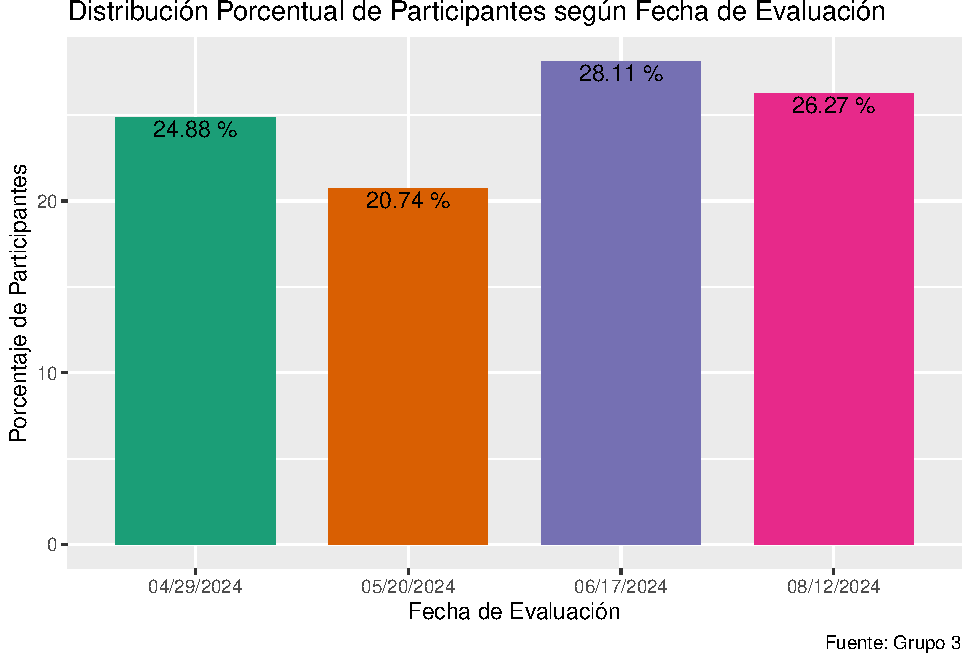
\includegraphics{Info_Dinix_02_files/figure-latex/30_Dem_FechAp-1.pdf}

\subsection{Edad en Meses}\label{edad-en-meses}

A continuación, la información acerca de la edad en meses del
participante

\begin{longtable}[]{@{}lrrrr@{}}
\caption{Frecuencias de Edad en Meses}\tabularnewline
\toprule\noalign{}
Edad en Meses & N & \% & N Acum. & \% Acum. \\
\midrule\noalign{}
\endfirsthead
\toprule\noalign{}
Edad en Meses & N & \% & N Acum. & \% Acum. \\
\midrule\noalign{}
\endhead
\bottomrule\noalign{}
\endlastfoot
32 & 1 & 0.09 & 1 & 0.09 \\
33 & 1 & 0.09 & 2 & 0.18 \\
36 & 5 & 0.46 & 7 & 0.64 \\
37 & 14 & 1.29 & 21 & 1.93 \\
38 & 33 & 3.04 & 54 & 4.97 \\
39 & 51 & 4.70 & 105 & 9.67 \\
40 & 58 & 5.35 & 163 & 15.02 \\
41 & 80 & 7.37 & 243 & 22.39 \\
42 & 79 & 7.28 & 322 & 29.67 \\
43 & 70 & 6.45 & 392 & 36.12 \\
44 & 74 & 6.82 & 466 & 42.94 \\
45 & 78 & 7.19 & 544 & 50.13 \\
46 & 91 & 8.39 & 635 & 58.52 \\
47 & 89 & 8.20 & 724 & 66.72 \\
48 & 97 & 8.94 & 821 & 75.66 \\
49 & 93 & 8.57 & 914 & 84.23 \\
50 & 62 & 5.71 & 976 & 89.94 \\
51 & 31 & 2.86 & 1007 & 92.80 \\
52 & 20 & 1.84 & 1027 & 94.64 \\
53 & 7 & 0.65 & 1034 & 95.29 \\
54 & 5 & 0.46 & 1039 & 95.75 \\
55 & 10 & 0.92 & 1049 & 96.67 \\
56 & 3 & 0.28 & 1052 & 96.95 \\
57 & 4 & 0.37 & 1056 & 97.32 \\
59 & 5 & 0.46 & 1061 & 97.78 \\
60 & 3 & 0.28 & 1064 & 98.06 \\
61 & 5 & 0.46 & 1069 & 98.52 \\
62 & 6 & 0.55 & 1075 & 99.07 \\
63 & 7 & 0.65 & 1082 & 99.72 \\
64 & 3 & 0.28 & 1085 & 100.00 \\
\end{longtable}

\begin{longtable}[]{@{}lrrrr@{}}
\toprule\noalign{}
Variable & Mediana & Media & Desviación.Estándar & Número.de.Casos \\
\midrule\noalign{}
\endhead
\bottomrule\noalign{}
\endlastfoot
Edad en Meses & 45 & 45.51 & 4.88 & 1085 \\
\end{longtable}

A continuación el histograma de la Edad en meses:

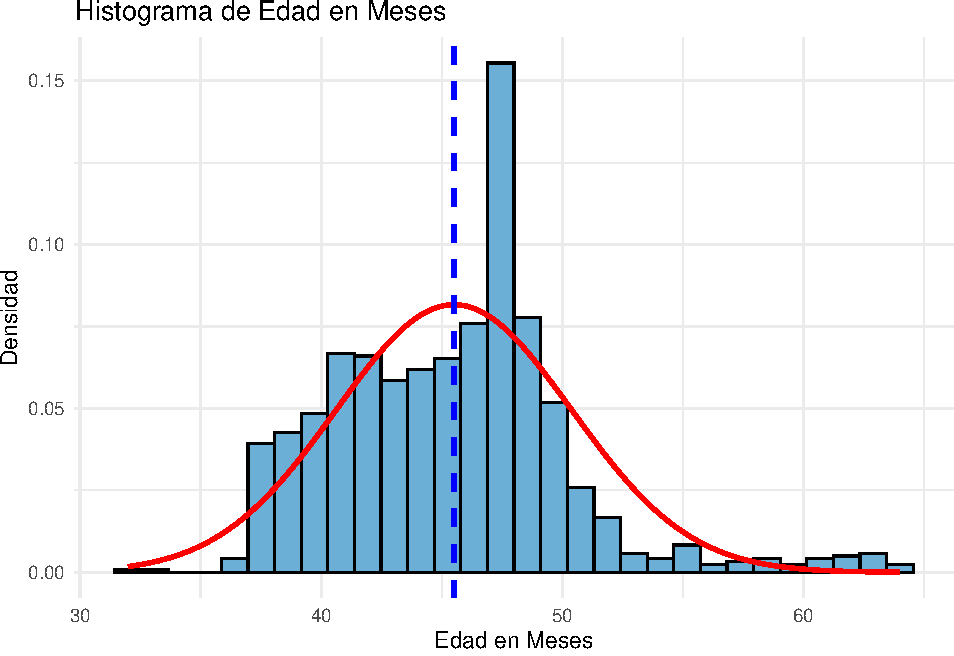
\includegraphics{Info_Dinix_02_files/figure-latex/30_AgeMo_Hist-1.pdf}

\subsection{Cuatrimestre de
Nacimiento}\label{cuatrimestre-de-nacimiento}

A continuación, la información acerca de la edad en meses del
participante. Esta variable fue creada a partir de los datos de fecha de
nacimiento de los participantes. El propósito es llegar a establecer,
posteriormente, si existe relación entre el cuatrimestre de nacimiento
del participante y el nivel de desempeño en la Escala DINI (relaciones
similares han sido encontradas en estudios previos para otros
instrumentos y mediciones de logro académico).

\begin{longtable}[]{@{}lrrrr@{}}
\caption{Frecuencias de Cuatrimestre}\tabularnewline
\toprule\noalign{}
Cuatrimestre & N & \% & N Acum. & \% Acum. \\
\midrule\noalign{}
\endfirsthead
\toprule\noalign{}
Cuatrimestre & N & \% & N Acum. & \% Acum. \\
\midrule\noalign{}
\endhead
\bottomrule\noalign{}
\endlastfoot
1 (Ene-Mar) & 222 & 20.46 & 222 & 20.46 \\
2 (Abr-Jun) & 342 & 31.52 & 564 & 51.98 \\
3 (Jul-Sep) & 276 & 25.44 & 840 & 77.42 \\
4 (Oct-Dic) & 245 & 22.58 & 1085 & 100.00 \\
\end{longtable}

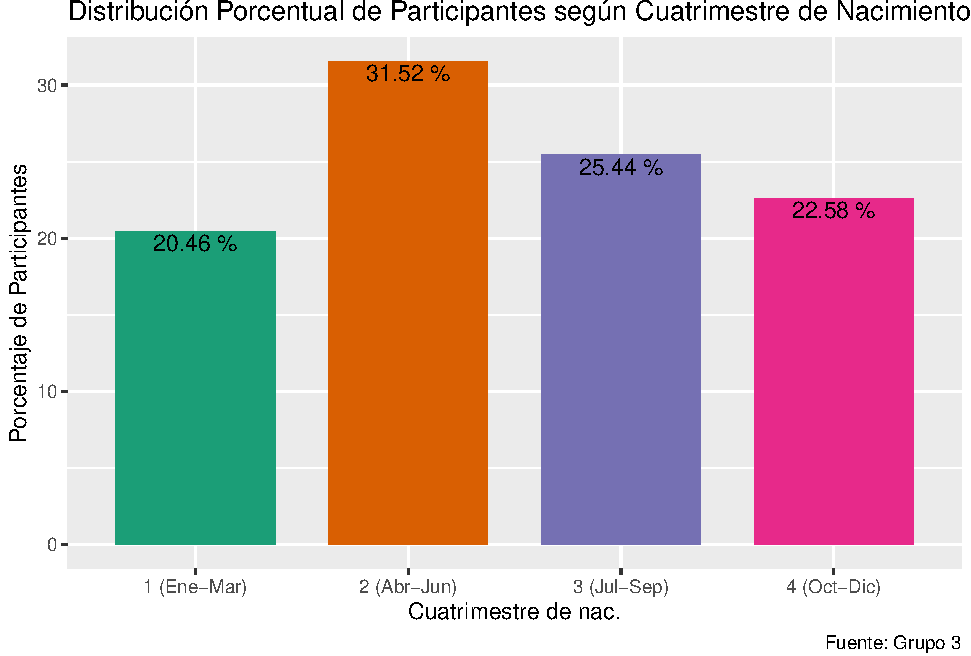
\includegraphics{Info_Dinix_02_files/figure-latex/30_QDOB-1.pdf}

\subsection{Código Modular}\label{cuxf3digo-modular}

A continuación, la información acerca del Código Modular

\begin{longtable}[]{@{}lrrrr@{}}
\caption{Frecuencias de Código Modular}\tabularnewline
\toprule\noalign{}
Código Modular & N & \% & N Acum. & \% Acum. \\
\midrule\noalign{}
\endfirsthead
\toprule\noalign{}
Código Modular & N & \% & N Acum. & \% Acum. \\
\midrule\noalign{}
\endhead
\bottomrule\noalign{}
\endlastfoot
0335422 & 75 & 6.91 & 75 & 6.91 \\
0838441 & 56 & 5.16 & 131 & 12.07 \\
0403964 & 55 & 5.07 & 186 & 17.14 \\
0259432 & 52 & 4.79 & 238 & 21.93 \\
0774372 & 51 & 4.70 & 289 & 26.63 \\
1504026 & 45 & 4.15 & 334 & 30.78 \\
1188184 & 44 & 4.06 & 378 & 34.84 \\
0565598 & 40 & 3.69 & 418 & 38.53 \\
0259630 & 39 & 3.59 & 457 & 42.12 \\
0259648 & 39 & 3.59 & 496 & 45.71 \\
0613646 & 39 & 3.59 & 535 & 49.30 \\
1321272 & 38 & 3.50 & 573 & 52.80 \\
0403659 & 33 & 3.04 & 606 & 55.84 \\
1630029 & 32 & 2.95 & 638 & 58.79 \\
0542175 & 31 & 2.86 & 669 & 61.65 \\
1152537 & 30 & 2.76 & 699 & 64.41 \\
0551192 & 25 & 2.30 & 724 & 66.71 \\
1055763 & 24 & 2.21 & 748 & 68.92 \\
0565952 & 23 & 2.12 & 771 & 71.04 \\
0259770 & 21 & 1.94 & 792 & 72.98 \\
0404079 & 19 & 1.75 & 811 & 74.73 \\
0500215 & 18 & 1.66 & 829 & 76.39 \\
0688838 & 18 & 1.66 & 847 & 78.05 \\
1137579 & 18 & 1.66 & 865 & 79.71 \\
0651901 & 15 & 1.38 & 880 & 81.09 \\
0930842 & 15 & 1.38 & 895 & 82.47 \\
1491182 & 15 & 1.38 & 910 & 83.85 \\
1396647 & 14 & 1.29 & 924 & 85.14 \\
0403675 & 13 & 1.20 & 937 & 86.34 \\
1516624 & 13 & 1.20 & 950 & 87.54 \\
0540062 & 11 & 1.01 & 961 & 88.55 \\
1674837 & 11 & 1.01 & 972 & 89.56 \\
1746148 & 11 & 1.01 & 983 & 90.57 \\
1556232 & 10 & 0.92 & 993 & 91.49 \\
3013380 & 10 & 0.92 & 1003 & 92.41 \\
1137942 & 9 & 0.83 & 1012 & 93.24 \\
1559608 & 8 & 0.74 & 1020 & 93.98 \\
3622240 & 8 & 0.74 & 1028 & 94.72 \\
1548437 & 7 & 0.65 & 1035 & 95.37 \\
0772780 & 6 & 0.55 & 1041 & 95.92 \\
0730275 & 5 & 0.46 & 1046 & 96.38 \\
1151570 & 5 & 0.46 & 1051 & 96.84 \\
1262419 & 5 & 0.46 & 1056 & 97.30 \\
1262773 & 4 & 0.37 & 1060 & 97.67 \\
1348036 & 4 & 0.37 & 1064 & 98.04 \\
1396605 & 3 & 0.28 & 1067 & 98.32 \\
1396720 & 3 & 0.28 & 1070 & 98.60 \\
1440577 & 3 & 0.28 & 1073 & 98.88 \\
1714815 & 3 & 0.28 & 1076 & 99.16 \\
0565606 & 2 & 0.18 & 1078 & 99.34 \\
0750604 & 2 & 0.18 & 1080 & 99.52 \\
1439017 & 2 & 0.18 & 1082 & 99.70 \\
1440627 & 2 & 0.18 & 1084 & 99.88 \\
0572446 & 1 & 0.09 & 1085 & 99.97 \\
\end{longtable}

\subsection{Región Natural}\label{regiuxf3n-natural}

A continuación, la información acerca de la Región Natural

\begin{longtable}[]{@{}lrrrr@{}}
\caption{Frecuencias de Regnat}\tabularnewline
\toprule\noalign{}
Regnat & N & \% & N Acum. & \% Acum. \\
\midrule\noalign{}
\endfirsthead
\toprule\noalign{}
Regnat & N & \% & N Acum. & \% Acum. \\
\midrule\noalign{}
\endhead
\bottomrule\noalign{}
\endlastfoot
Costa & 489 & 45.07 & 489 & 45.07 \\
Sierra & 277 & 25.53 & 766 & 70.60 \\
Selva & 319 & 29.40 & 1085 & 100.00 \\
\end{longtable}

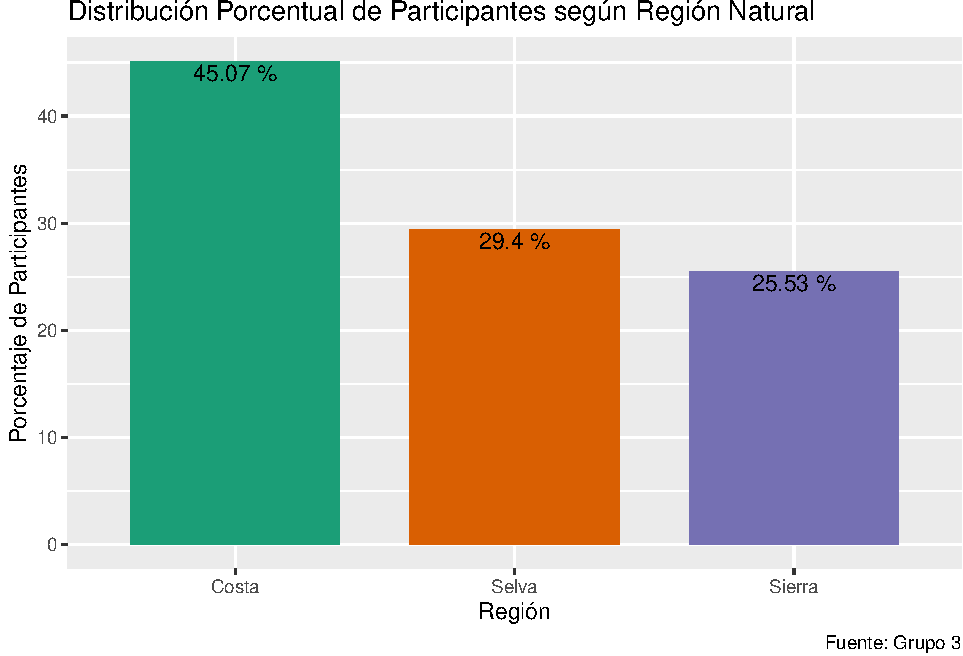
\includegraphics{Info_Dinix_02_files/figure-latex/30_RegNat-1.pdf}

\subsection{Área}\label{uxe1rea}

A continuación, la información acerca del Área

\begin{longtable}[]{@{}lrrrr@{}}
\caption{Frecuencias de Area}\tabularnewline
\toprule\noalign{}
Area & N & \% & N Acum. & \% Acum. \\
\midrule\noalign{}
\endfirsthead
\toprule\noalign{}
Area & N & \% & N Acum. & \% Acum. \\
\midrule\noalign{}
\endhead
\bottomrule\noalign{}
\endlastfoot
Urbana & 776 & 71.52 & 776 & 71.52 \\
Rural & 309 & 28.48 & 1085 & 100.00 \\
\end{longtable}

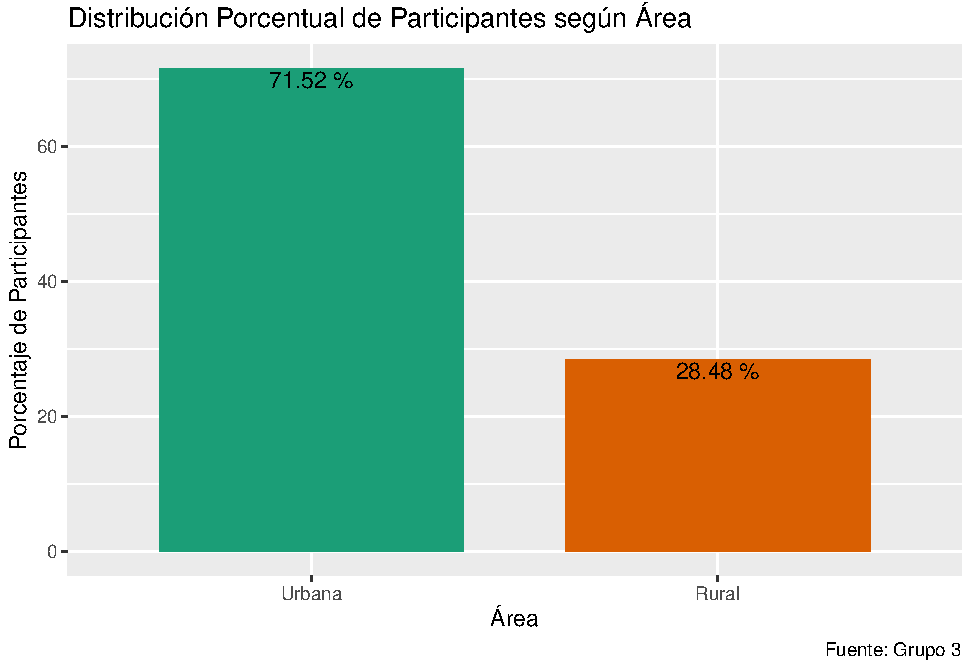
\includegraphics{Info_Dinix_02_files/figure-latex/30_Area-1.pdf}

\subsection{Nivel Modalidad}\label{nivel-modalidad}

A continuación, la información acerca del Nivel Modalidad

\begin{longtable}[]{@{}lrrrr@{}}
\caption{Frecuencias de Nivel Modalidad}\tabularnewline
\toprule\noalign{}
Nivel Modalidad & N & \% & N Acum. & \% Acum. \\
\midrule\noalign{}
\endfirsthead
\toprule\noalign{}
Nivel Modalidad & N & \% & N Acum. & \% Acum. \\
\midrule\noalign{}
\endhead
\bottomrule\noalign{}
\endlastfoot
Inicial - Jardín & 893 & 82.30 & 893 & 82.30 \\
Inicial - Cuna-jardín & 184 & 16.96 & 1077 & 99.26 \\
Inicial - Programa no escolarizado & 8 & 0.74 & 1085 & 100.00 \\
\end{longtable}

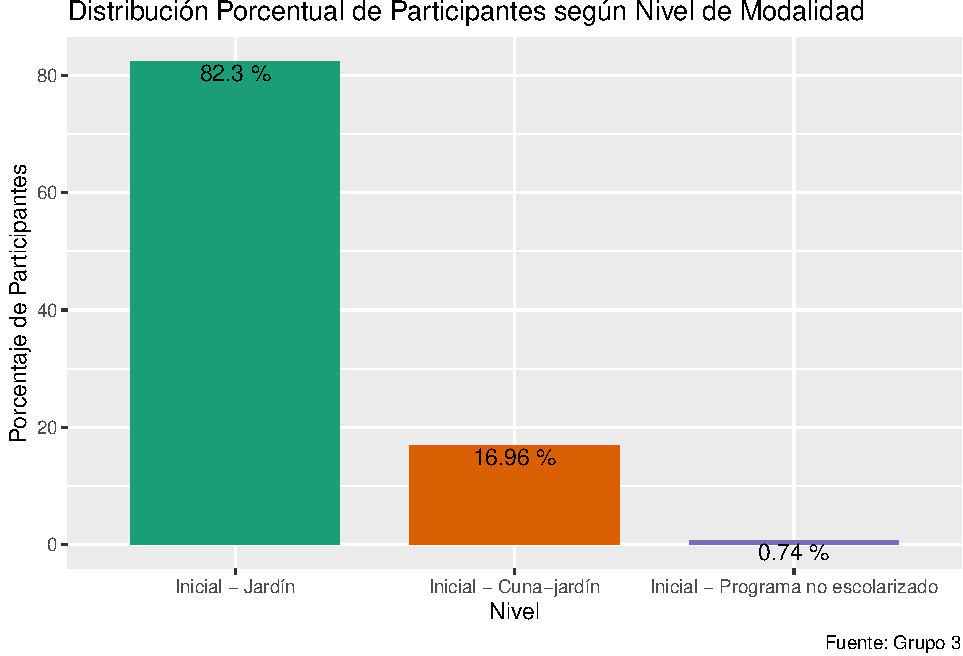
\includegraphics{Info_Dinix_02_files/figure-latex/30_NivMod-1.pdf}

\subsection{Gestión}\label{gestiuxf3n}

A continuación, la información acerca de la Gestión (Pública o Privada)
de la institución edicativa.

\begin{longtable}[]{@{}lrrrr@{}}
\caption{Frecuencias de Gestión}\tabularnewline
\toprule\noalign{}
Gestión & N & \% & N Acum. & \% Acum. \\
\midrule\noalign{}
\endfirsthead
\toprule\noalign{}
Gestión & N & \% & N Acum. & \% Acum. \\
\midrule\noalign{}
\endhead
\bottomrule\noalign{}
\endlastfoot
Pública & 967 & 89.12 & 967 & 89.12 \\
Privada & 118 & 10.88 & 1085 & 100.00 \\
\end{longtable}

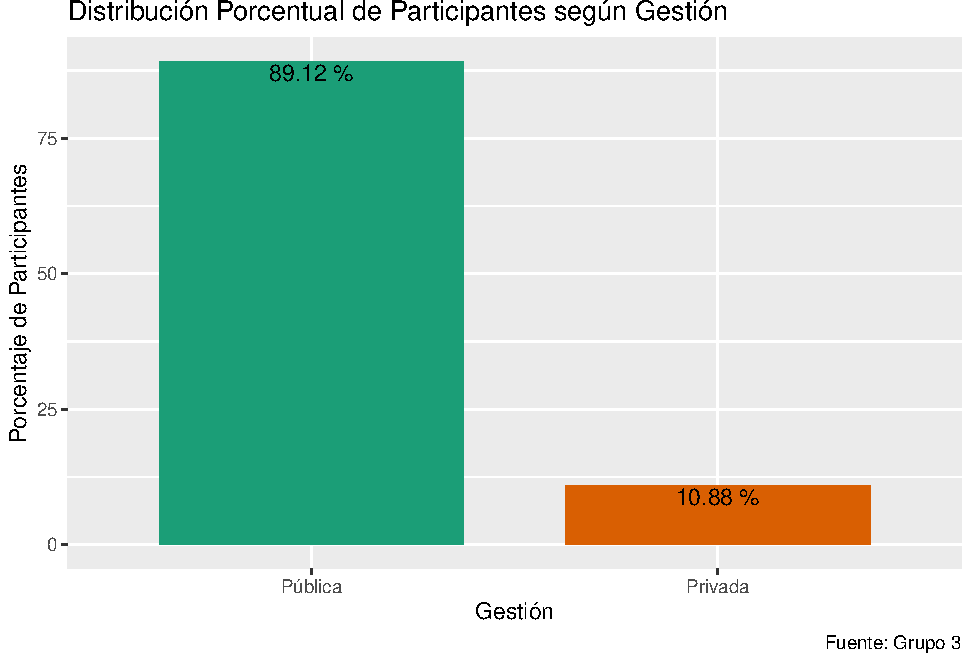
\includegraphics{Info_Dinix_02_files/figure-latex/30_Gest-1.pdf}

\subsection{Departamento}\label{departamento}

A continuación, la información acerca del Departamento en donde vive el
participante.

\begin{longtable}[]{@{}lrrrr@{}}
\caption{Frecuencias de Departamento}\tabularnewline
\toprule\noalign{}
Departamento & N & \% & N Acum. & \% Acum. \\
\midrule\noalign{}
\endfirsthead
\toprule\noalign{}
Departamento & N & \% & N Acum. & \% Acum. \\
\midrule\noalign{}
\endhead
\bottomrule\noalign{}
\endlastfoot
Piura & 305 & 28.11 & 305 & 28.11 \\
Lima Metropolitana & 285 & 26.27 & 590 & 54.38 \\
Cusco & 270 & 24.88 & 860 & 79.26 \\
Loreto & 225 & 20.74 & 1085 & 100.00 \\
\end{longtable}

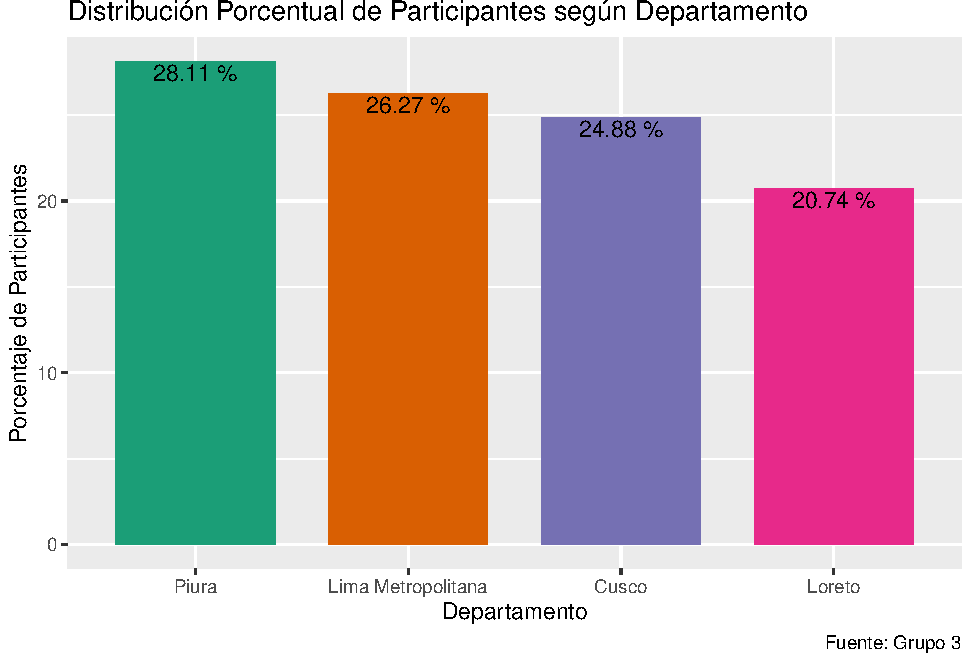
\includegraphics{Info_Dinix_02_files/figure-latex/30_Depa-1.pdf}

\subsection{Quintil de Pobreza}\label{quintil-de-pobreza}

A continuación, la información acerca del Departamento en donde vive el
participante.

\begin{longtable}[]{@{}lrrrr@{}}
\caption{Frecuencias de Quintil}\tabularnewline
\toprule\noalign{}
Quintil & N & \% & N Acum. & \% Acum. \\
\midrule\noalign{}
\endfirsthead
\toprule\noalign{}
Quintil & N & \% & N Acum. & \% Acum. \\
\midrule\noalign{}
\endhead
\bottomrule\noalign{}
\endlastfoot
1 & 137 & 12.63 & 137 & 12.63 \\
2 & 90 & 8.29 & 227 & 20.92 \\
3 & 198 & 18.25 & 425 & 39.17 \\
4 & 392 & 36.13 & 817 & 75.30 \\
5 & 268 & 24.70 & 1085 & 100.00 \\
\end{longtable}

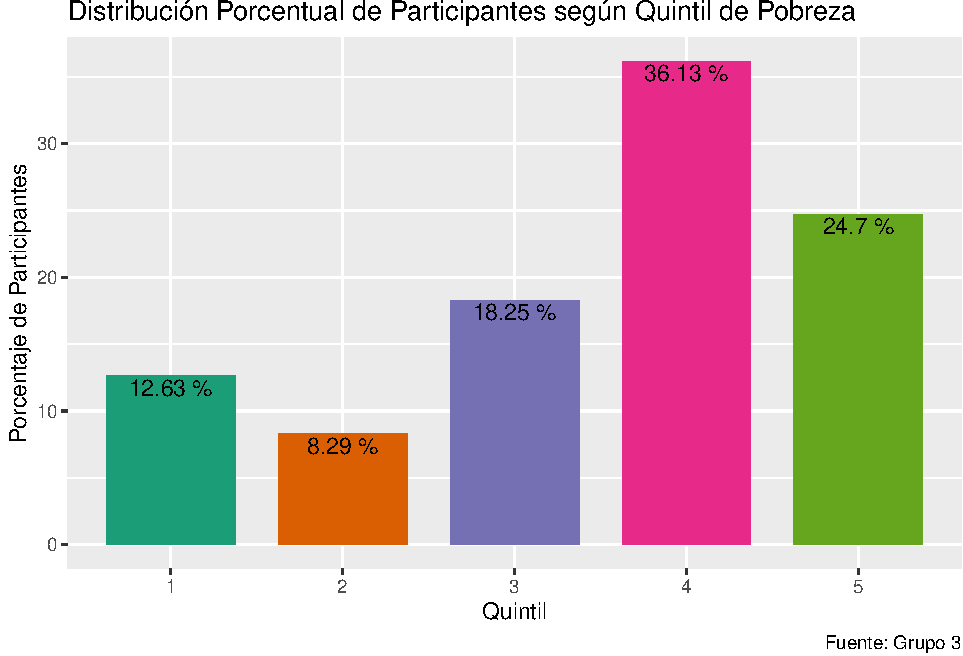
\includegraphics{Info_Dinix_02_files/figure-latex/30_Quintus-1.pdf}

\subsection{Incidencia / No Incidencia
(VSS)}\label{incidencia-no-incidencia-vss}

A continuación, la información acerca de la Incidencia / No Incidencia.

\begin{longtable}[]{@{}lrrrr@{}}
\caption{Frecuencias de Incidencia}\tabularnewline
\toprule\noalign{}
Incidencia & N & \% & N Acum. & \% Acum. \\
\midrule\noalign{}
\endfirsthead
\toprule\noalign{}
Incidencia & N & \% & N Acum. & \% Acum. \\
\midrule\noalign{}
\endhead
\bottomrule\noalign{}
\endlastfoot
No & 976 & 89.95 & 976 & 89.95 \\
Sí & 109 & 10.05 & 1085 & 100.00 \\
\end{longtable}

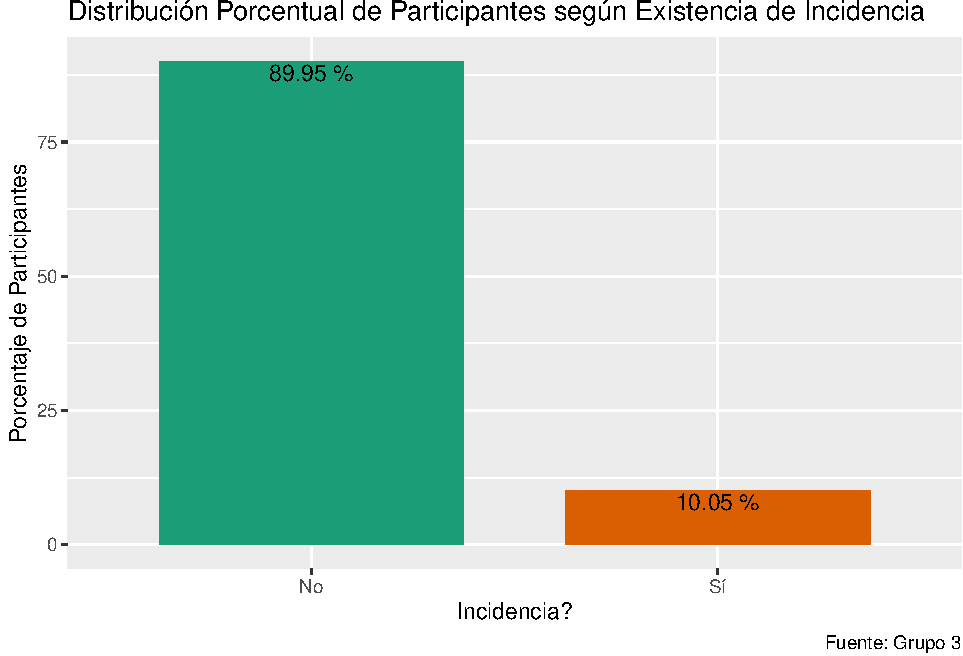
\includegraphics{Info_Dinix_02_files/figure-latex/30_VSS-1.pdf}

\subsection{Incidencia Perinatal
(VSSdesper)}\label{incidencia-perinatal-vssdesper}

A continuación, la información acerca de la Incidencia Perinatal.

\begin{longtable}[]{@{}lrrrr@{}}
\caption{Frecuencias de Incidencia Perinatal}\tabularnewline
\toprule\noalign{}
Incidencia Perinatal & N & \% & N Acum. & \% Acum. \\
\midrule\noalign{}
\endfirsthead
\toprule\noalign{}
Incidencia Perinatal & N & \% & N Acum. & \% Acum. \\
\midrule\noalign{}
\endhead
\bottomrule\noalign{}
\endlastfoot
No & 1067 & 98.34 & 1067 & 98.34 \\
Sí & 18 & 1.66 & 1085 & 100.00 \\
\end{longtable}

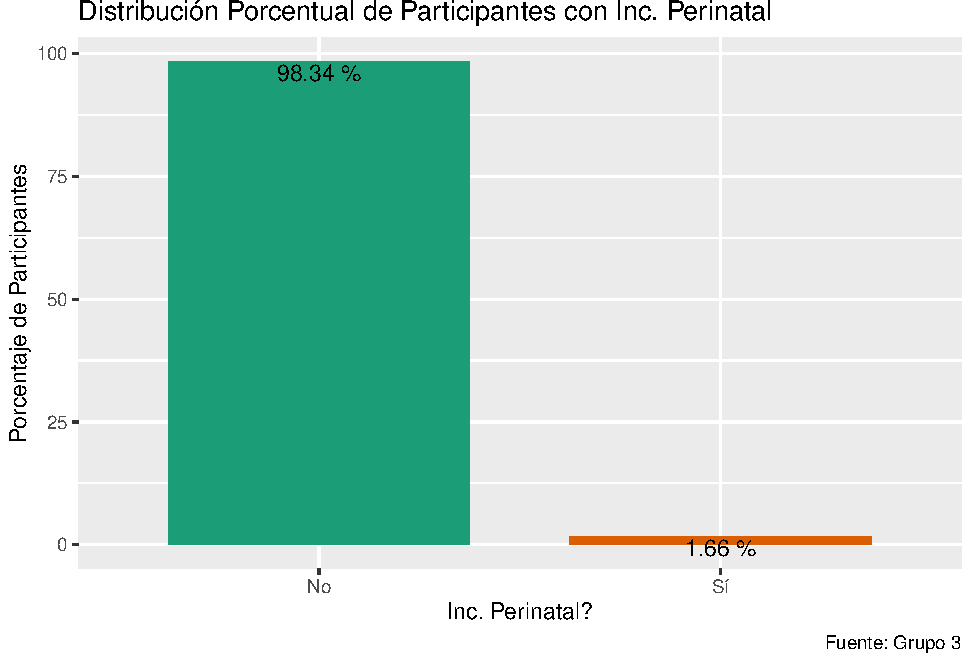
\includegraphics{Info_Dinix_02_files/figure-latex/30_VSSdesper-1.pdf}

\subsection{Incidencia Tratamiento Médico
(VSSttomed)}\label{incidencia-tratamiento-muxe9dico-vssttomed}

A continuación, la información acerca de la Incidencia por Tratamiento
Médico.

\begin{longtable}[]{@{}lrrrr@{}}
\caption{Frecuencias de Tto. Médico}\tabularnewline
\toprule\noalign{}
Tto. Médico & N & \% & N Acum. & \% Acum. \\
\midrule\noalign{}
\endfirsthead
\toprule\noalign{}
Tto. Médico & N & \% & N Acum. & \% Acum. \\
\midrule\noalign{}
\endhead
\bottomrule\noalign{}
\endlastfoot
No & 1067 & 98.34 & 1067 & 98.34 \\
Sí & 18 & 1.66 & 1085 & 100.00 \\
\end{longtable}

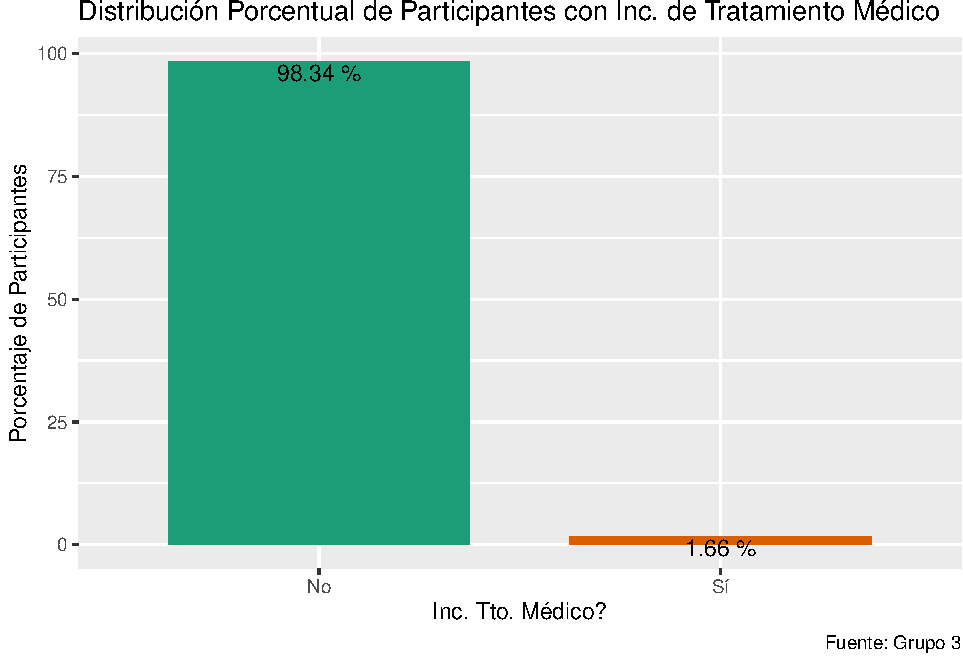
\includegraphics{Info_Dinix_02_files/figure-latex/30_VSSttomed-1.pdf}

\subsection{Incidencia por Patología
(VSSpatolo)}\label{incidencia-por-patologuxeda-vsspatolo}

A continuación, la información acerca de la Incidencia por Patología.

\begin{longtable}[]{@{}lrrrr@{}}
\caption{Frecuencias de Patología}\tabularnewline
\toprule\noalign{}
Patología & N & \% & N Acum. & \% Acum. \\
\midrule\noalign{}
\endfirsthead
\toprule\noalign{}
Patología & N & \% & N Acum. & \% Acum. \\
\midrule\noalign{}
\endhead
\bottomrule\noalign{}
\endlastfoot
No & 1078 & 99.35 & 1078 & 99.35 \\
Sí & 7 & 0.65 & 1085 & 100.00 \\
\end{longtable}

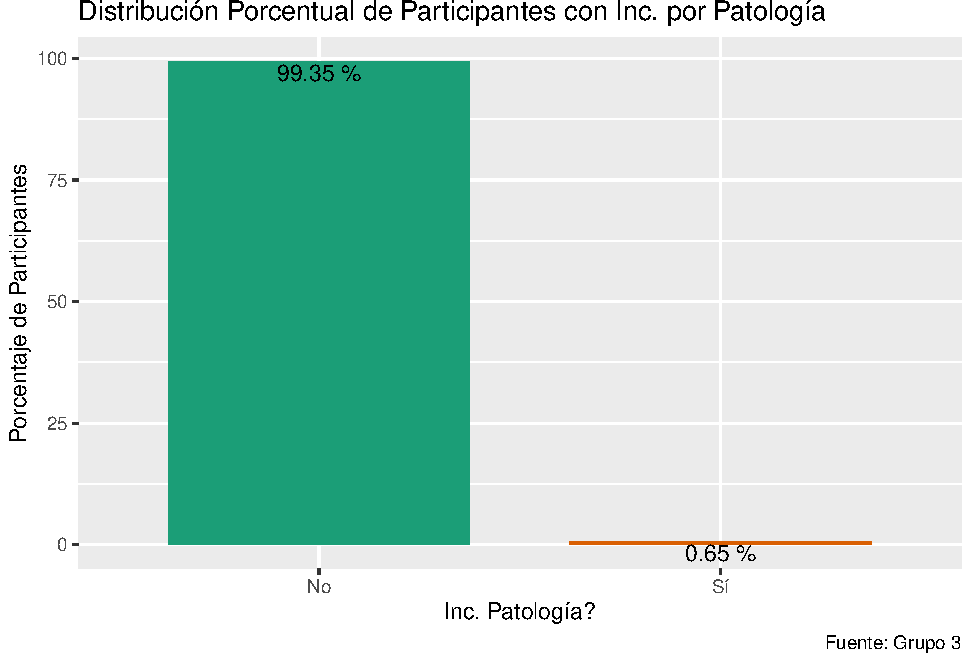
\includegraphics{Info_Dinix_02_files/figure-latex/30_VSSpatolo-1.pdf}

\subsection{Incidencia por Negligencia
(VSSnegl)}\label{incidencia-por-negligencia-vssnegl}

A continuación, la información acerca de la Incidencia por Negligencia

\begin{longtable}[]{@{}lrrrr@{}}
\caption{Frecuencias de Negligencia}\tabularnewline
\toprule\noalign{}
Negligencia & N & \% & N Acum. & \% Acum. \\
\midrule\noalign{}
\endfirsthead
\toprule\noalign{}
Negligencia & N & \% & N Acum. & \% Acum. \\
\midrule\noalign{}
\endhead
\bottomrule\noalign{}
\endlastfoot
No & 1080 & 99.54 & 1080 & 99.54 \\
Sí & 5 & 0.46 & 1085 & 100.00 \\
\end{longtable}

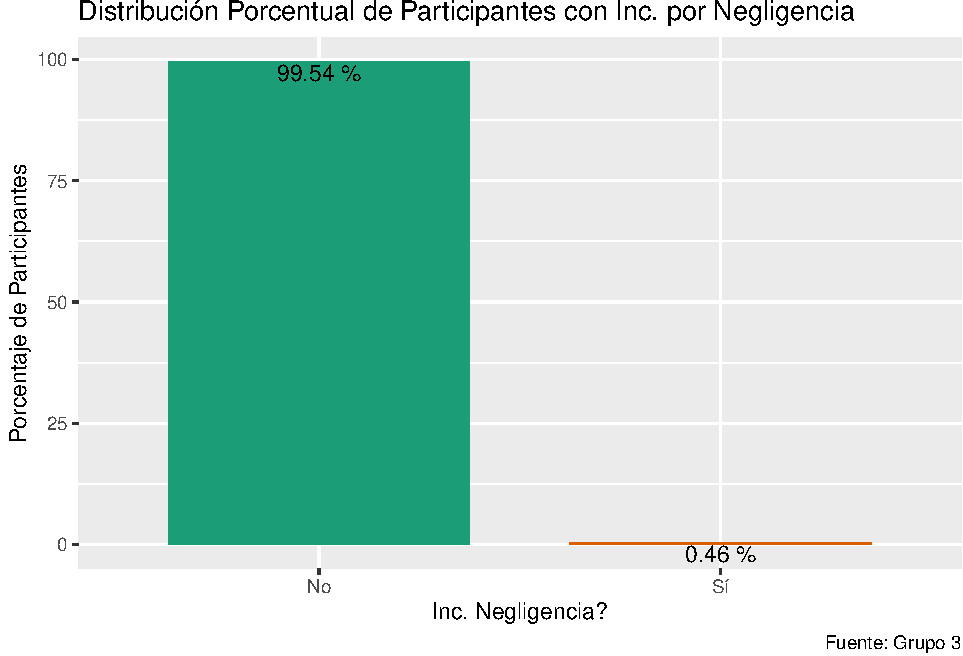
\includegraphics{Info_Dinix_02_files/figure-latex/30_VSSnegl-1.pdf}

\subsection{Incidencia por Mudanza
(VSSmud)}\label{incidencia-por-mudanza-vssmud}

A continuación, la información acerca de la Incidencia por Mudanza

\begin{longtable}[]{@{}lrrrr@{}}
\caption{Frecuencias de Inc.~Mudanza}\tabularnewline
\toprule\noalign{}
Inc.~Mudanza & N & \% & N Acum. & \% Acum. \\
\midrule\noalign{}
\endfirsthead
\toprule\noalign{}
Inc.~Mudanza & N & \% & N Acum. & \% Acum. \\
\midrule\noalign{}
\endhead
\bottomrule\noalign{}
\endlastfoot
No & 1055 & 97.24 & 1055 & 97.24 \\
Sí & 30 & 2.76 & 1085 & 100.00 \\
\end{longtable}

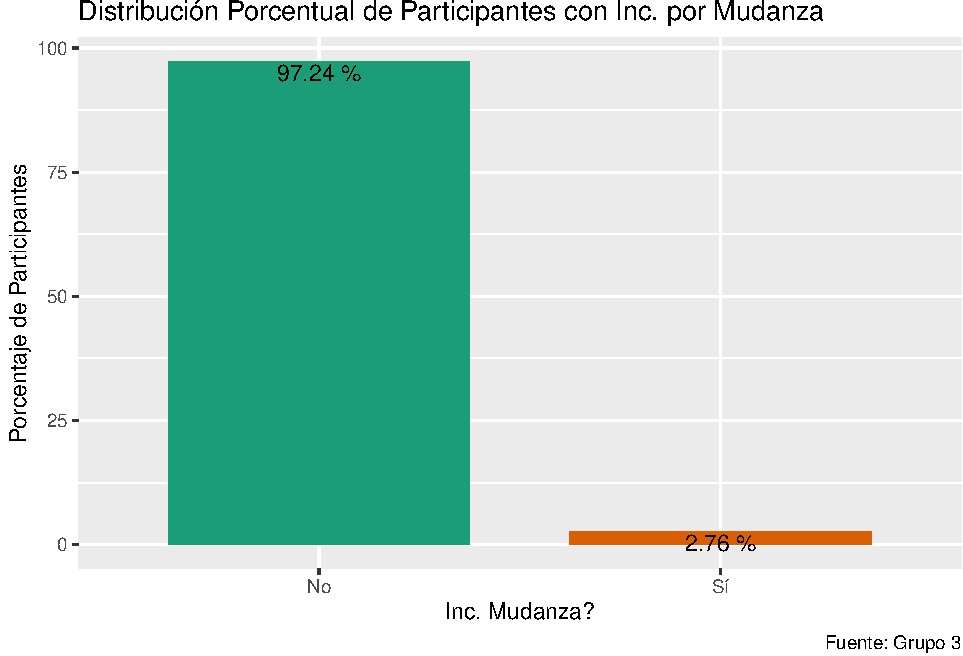
\includegraphics{Info_Dinix_02_files/figure-latex/30_VSSmud-1.pdf}

\subsection{Incidencia por Consumo
(VSSconsus)}\label{incidencia-por-consumo-vssconsus}

A continuación, la información acerca de la Incidencia por Consumo:

\begin{longtable}[]{@{}lrrrr@{}}
\caption{Frecuencias de Inc.~Consumo}\tabularnewline
\toprule\noalign{}
Inc.~Consumo & N & \% & N Acum. & \% Acum. \\
\midrule\noalign{}
\endfirsthead
\toprule\noalign{}
Inc.~Consumo & N & \% & N Acum. & \% Acum. \\
\midrule\noalign{}
\endhead
\bottomrule\noalign{}
\endlastfoot
No & 1080 & 99.54 & 1080 & 99.54 \\
Sí & 5 & 0.46 & 1085 & 100.00 \\
\end{longtable}

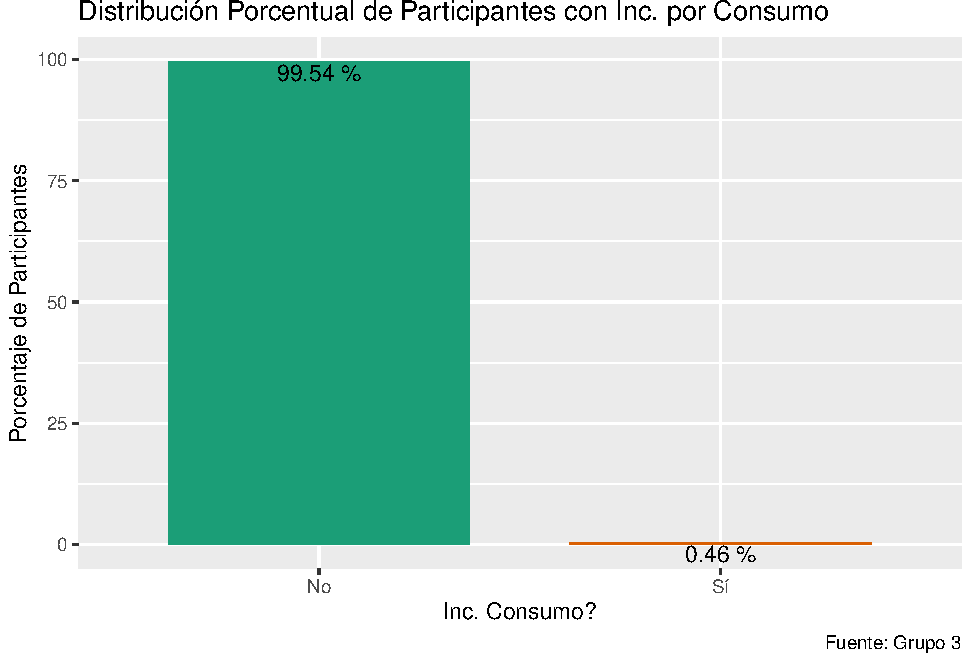
\includegraphics{Info_Dinix_02_files/figure-latex/30_VSSconsus-1.pdf}

\subsection{Incidencia por Desempleo
(VSSdesemp)}\label{incidencia-por-desempleo-vssdesemp}

A continuación, la información acerca de la Incidencia por Desempleo:

\begin{longtable}[]{@{}lrrrr@{}}
\caption{Frecuencias de Inc.~por Desempleo}\tabularnewline
\toprule\noalign{}
Inc.~por Desempleo & N & \% & N Acum. & \% Acum. \\
\midrule\noalign{}
\endfirsthead
\toprule\noalign{}
Inc.~por Desempleo & N & \% & N Acum. & \% Acum. \\
\midrule\noalign{}
\endhead
\bottomrule\noalign{}
\endlastfoot
No & 1061 & 97.79 & 1061 & 97.79 \\
Sí & 24 & 2.21 & 1085 & 100.00 \\
\end{longtable}

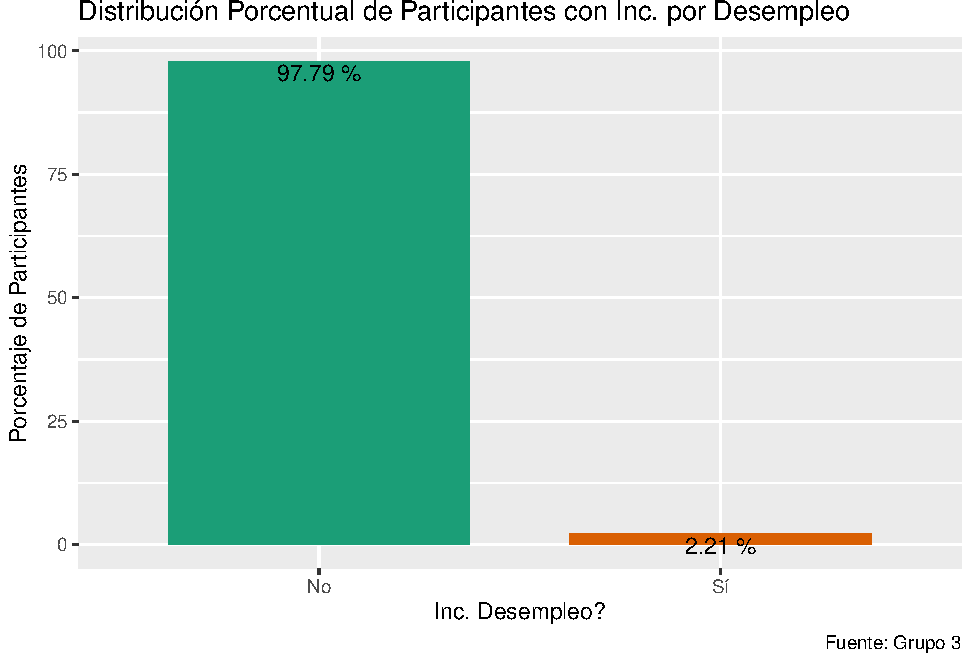
\includegraphics{Info_Dinix_02_files/figure-latex/30_VSSdesemp-1.pdf}

\subsection{Incidencia Familiar
(VSSfamprilib)}\label{incidencia-familiar-vssfamprilib}

A continuación, la información acerca de la Incidencia Familiar:

\begin{longtable}[]{@{}lrrrr@{}}
\caption{Frecuencias de Inc.~Familiar}\tabularnewline
\toprule\noalign{}
Inc.~Familiar & N & \% & N Acum. & \% Acum. \\
\midrule\noalign{}
\endfirsthead
\toprule\noalign{}
Inc.~Familiar & N & \% & N Acum. & \% Acum. \\
\midrule\noalign{}
\endhead
\bottomrule\noalign{}
\endlastfoot
No & 1084 & 99.91 & 1084 & 99.91 \\
Sí & 1 & 0.09 & 1085 & 100.00 \\
\end{longtable}

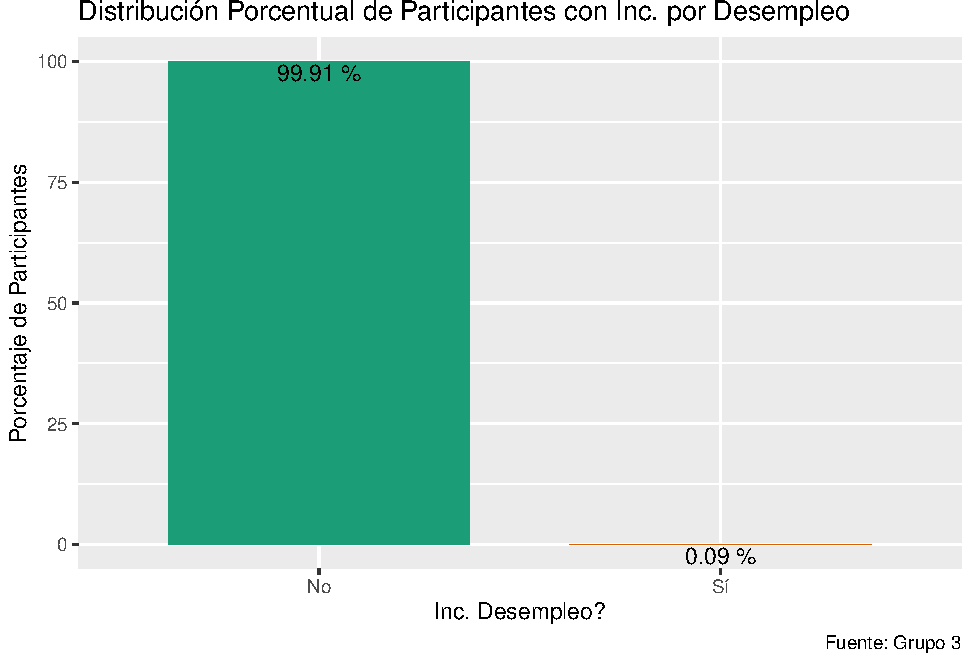
\includegraphics{Info_Dinix_02_files/figure-latex/30_VSSfamprilib-1.pdf}

\subsection{Incidencia Otros (VSSotro)}\label{incidencia-otros-vssotro}

A continuación, la información acerca de la Incidencia Otros:

\begin{longtable}[]{@{}lrrrr@{}}
\caption{Frecuencias de Inc.~Otros}\tabularnewline
\toprule\noalign{}
Inc.~Otros & N & \% & N Acum. & \% Acum. \\
\midrule\noalign{}
\endfirsthead
\toprule\noalign{}
Inc.~Otros & N & \% & N Acum. & \% Acum. \\
\midrule\noalign{}
\endhead
\bottomrule\noalign{}
\endlastfoot
No & 1033 & 95.21 & 1033 & 95.21 \\
Sí & 52 & 4.79 & 1085 & 100.00 \\
\end{longtable}

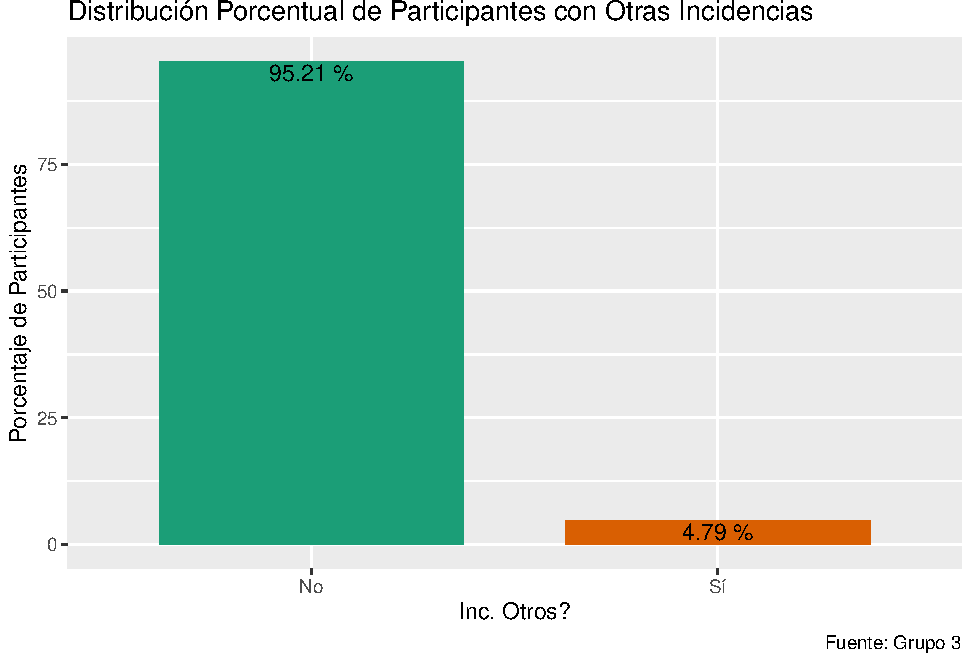
\includegraphics{Info_Dinix_02_files/figure-latex/30_VSSotro-1.pdf}

\subsection{Tratamiento Técnico (RTT)}\label{tratamiento-tuxe9cnico-rtt}

A continuación, la información acerca de Tratamiento Técnico:

\begin{longtable}[]{@{}lrrrr@{}}
\caption{Frecuencias de Tto. Técnico}\tabularnewline
\toprule\noalign{}
Tto. Técnico & N & \% & N Acum. & \% Acum. \\
\midrule\noalign{}
\endfirsthead
\toprule\noalign{}
Tto. Técnico & N & \% & N Acum. & \% Acum. \\
\midrule\noalign{}
\endhead
\bottomrule\noalign{}
\endlastfoot
No & 1056 & 97.33 & 1056 & 97.33 \\
Sí & 29 & 2.67 & 1085 & 100.00 \\
\end{longtable}

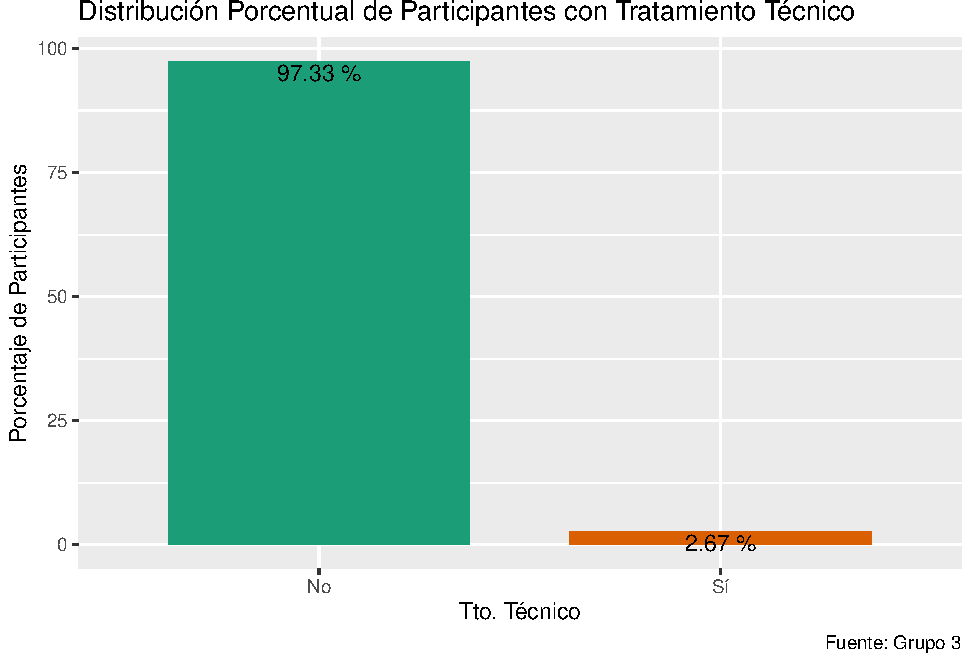
\includegraphics{Info_Dinix_02_files/figure-latex/30_RTT-1.pdf}

\subsection{Tratamiento Psicológico
(RTTasipsi)}\label{tratamiento-psicoluxf3gico-rttasipsi}

A continuación, la información acerca de Tratamiento Psicológico:

\begin{longtable}[]{@{}lrrrr@{}}
\caption{Frecuencias de Tto. Psicológico}\tabularnewline
\toprule\noalign{}
Tto. Psicológico & N & \% & N Acum. & \% Acum. \\
\midrule\noalign{}
\endfirsthead
\toprule\noalign{}
Tto. Psicológico & N & \% & N Acum. & \% Acum. \\
\midrule\noalign{}
\endhead
\bottomrule\noalign{}
\endlastfoot
No & 1061 & 97.79 & 1061 & 97.79 \\
Sí & 24 & 2.21 & 1085 & 100.00 \\
\end{longtable}

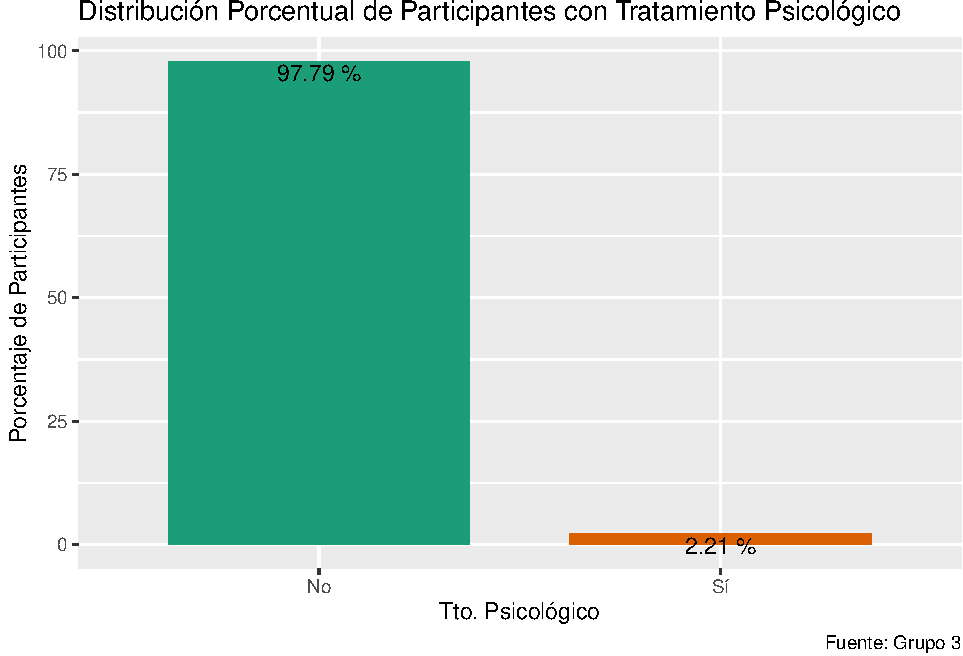
\includegraphics{Info_Dinix_02_files/figure-latex/30_RTTasipsi-1.pdf}

\subsection{Tratamiento Psiquiátrico
(RTTasipsiq)}\label{tratamiento-psiquiuxe1trico-rttasipsiq}

A continuación, la información acerca de Tratamiento Psiquiátrico:

\begin{longtable}[]{@{}lrrrr@{}}
\caption{Frecuencias de Tto. Psiquiátrico}\tabularnewline
\toprule\noalign{}
Tto. Psiquiátrico & N & \% & N Acum. & \% Acum. \\
\midrule\noalign{}
\endfirsthead
\toprule\noalign{}
Tto. Psiquiátrico & N & \% & N Acum. & \% Acum. \\
\midrule\noalign{}
\endhead
\bottomrule\noalign{}
\endlastfoot
No & 1082 & 99.72 & 1082 & 99.72 \\
Sí & 3 & 0.28 & 1085 & 100.00 \\
\end{longtable}

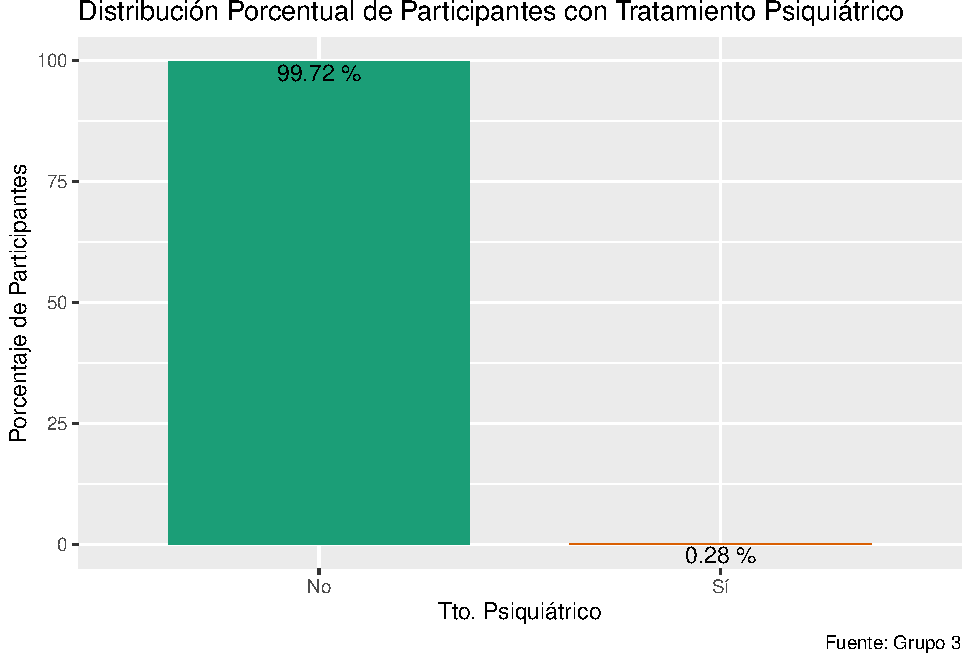
\includegraphics{Info_Dinix_02_files/figure-latex/30_RTTasipsiq-1.pdf}

\subsection{Tratamiento Pedagógico
(RTTasiped)}\label{tratamiento-pedaguxf3gico-rttasiped}

A continuación, la información acerca de Tratamiento Pedagógico:

\begin{longtable}[]{@{}lrrrr@{}}
\caption{Frecuencias de Tto. Pedagógico}\tabularnewline
\toprule\noalign{}
Tto. Pedagógico & N & \% & N Acum. & \% Acum. \\
\midrule\noalign{}
\endfirsthead
\toprule\noalign{}
Tto. Pedagógico & N & \% & N Acum. & \% Acum. \\
\midrule\noalign{}
\endhead
\bottomrule\noalign{}
\endlastfoot
No & 1065 & 98.16 & 1065 & 98.16 \\
Sí & 20 & 1.84 & 1085 & 100.00 \\
\end{longtable}

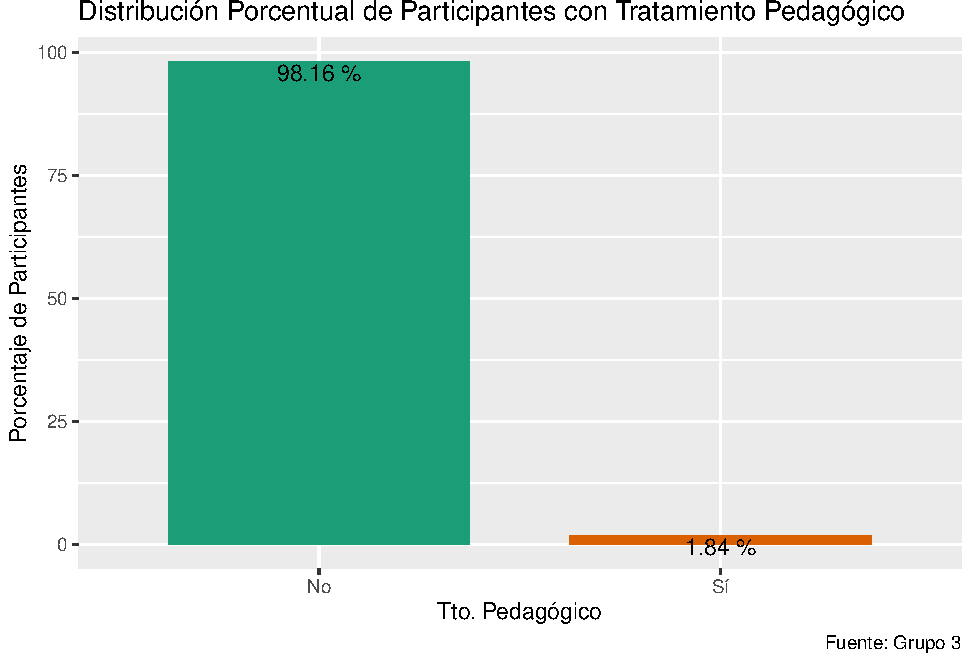
\includegraphics{Info_Dinix_02_files/figure-latex/30_RTTasiped-1.pdf}

\subsection{Tratamiento Psicomotriz
(RTTasipsim)}\label{tratamiento-psicomotriz-rttasipsim}

A continuación, la información acerca de Tratamiento Psicomotriz:

\begin{longtable}[]{@{}lrrrr@{}}
\caption{Frecuencias de Tto. Psicomotriz}\tabularnewline
\toprule\noalign{}
Tto. Psicomotriz & N & \% & N Acum. & \% Acum. \\
\midrule\noalign{}
\endfirsthead
\toprule\noalign{}
Tto. Psicomotriz & N & \% & N Acum. & \% Acum. \\
\midrule\noalign{}
\endhead
\bottomrule\noalign{}
\endlastfoot
No & 1063 & 97.97 & 1063 & 97.97 \\
Sí & 22 & 2.03 & 1085 & 100.00 \\
\end{longtable}

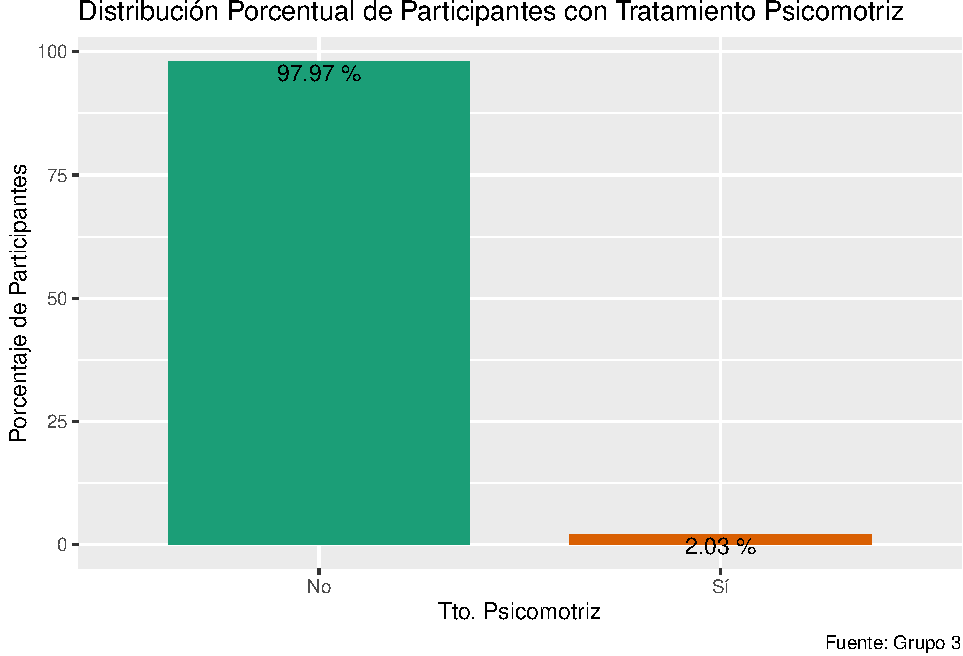
\includegraphics{Info_Dinix_02_files/figure-latex/30_RTTasipsim-1.pdf}

\subsection{Tratamiento Fonoaudiológico
(RTTasifon)}\label{tratamiento-fonoaudioluxf3gico-rttasifon}

A continuación, la información acerca de Tratamiento Fonoaudiológico:

\begin{longtable}[]{@{}lrrrr@{}}
\caption{Frecuencias de Tto. Fonoaudiológico}\tabularnewline
\toprule\noalign{}
Tto. Fonoaudiológico & N & \% & N Acum. & \% Acum. \\
\midrule\noalign{}
\endfirsthead
\toprule\noalign{}
Tto. Fonoaudiológico & N & \% & N Acum. & \% Acum. \\
\midrule\noalign{}
\endhead
\bottomrule\noalign{}
\endlastfoot
No & 1069 & 98.53 & 1069 & 98.53 \\
Sí & 16 & 1.47 & 1085 & 100.00 \\
\end{longtable}

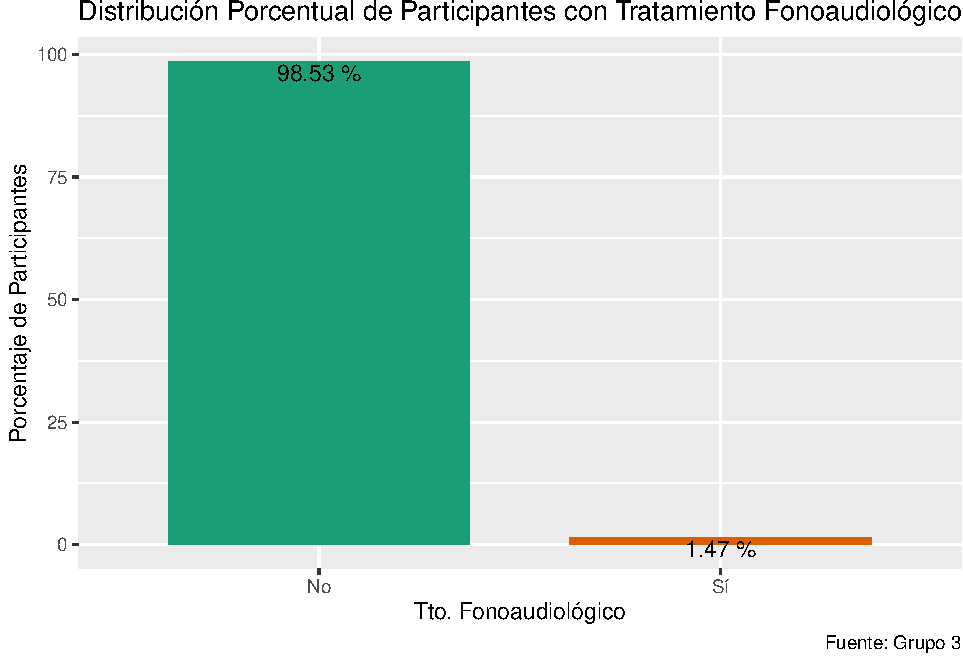
\includegraphics{Info_Dinix_02_files/figure-latex/30_RTTasifon-1.pdf}

\subsection{Tratamiento por Dificultades Diagnosticadas
(RTTdifdiag)}\label{tratamiento-por-dificultades-diagnosticadas-rttdifdiag}

A continuación, la información acerca de Tratamiento por Dificultades
Diagnosticadas:

\begin{longtable}[]{@{}lrrrr@{}}
\caption{Frecuencias de Tto. por Dif. Diag.}\tabularnewline
\toprule\noalign{}
Tto. por Dif. Diag. & N & \% & N Acum. & \% Acum. \\
\midrule\noalign{}
\endfirsthead
\toprule\noalign{}
Tto. por Dif. Diag. & N & \% & N Acum. & \% Acum. \\
\midrule\noalign{}
\endhead
\bottomrule\noalign{}
\endlastfoot
No & 1084 & 99.91 & 1084 & 99.91 \\
Sí & 1 & 0.09 & 1085 & 100.00 \\
\end{longtable}

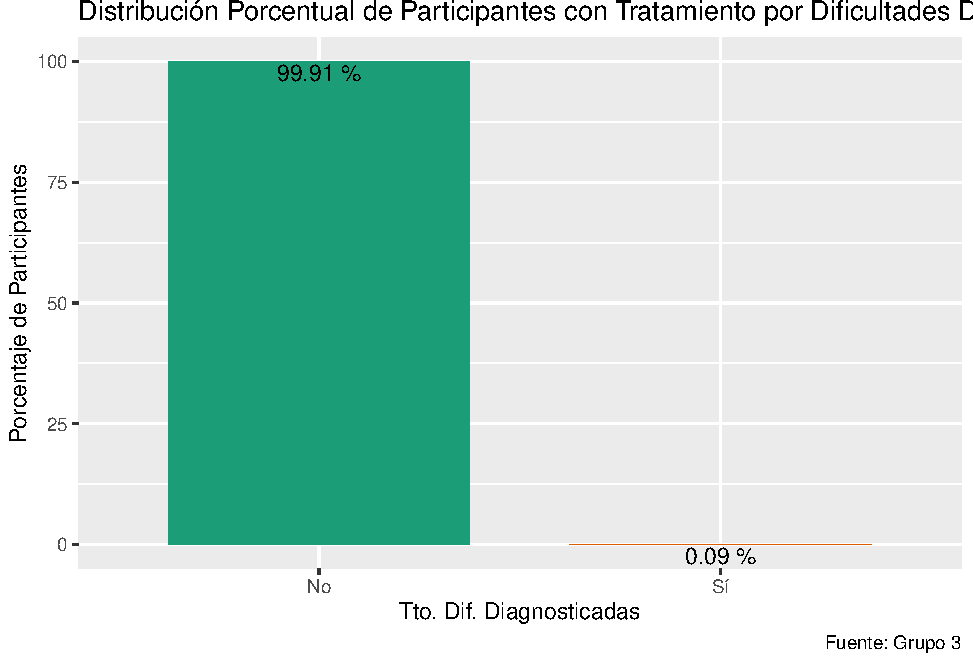
\includegraphics{Info_Dinix_02_files/figure-latex/30_RTTdifdiag-1.pdf}

\subsection{Tratamiento por Discapacidad
(RTTdisc)}\label{tratamiento-por-discapacidad-rttdisc}

A continuación, la información acerca de Tratamiento por Discapacidad:

\begin{longtable}[]{@{}lrrrr@{}}
\caption{Frecuencias de Tto. por Discapacidad}\tabularnewline
\toprule\noalign{}
Tto. por Discapacidad & N & \% & N Acum. & \% Acum. \\
\midrule\noalign{}
\endfirsthead
\toprule\noalign{}
Tto. por Discapacidad & N & \% & N Acum. & \% Acum. \\
\midrule\noalign{}
\endhead
\bottomrule\noalign{}
\endlastfoot
No & 1082 & 99.72 & 1082 & 99.72 \\
Sí & 3 & 0.28 & 1085 & 100.00 \\
\end{longtable}

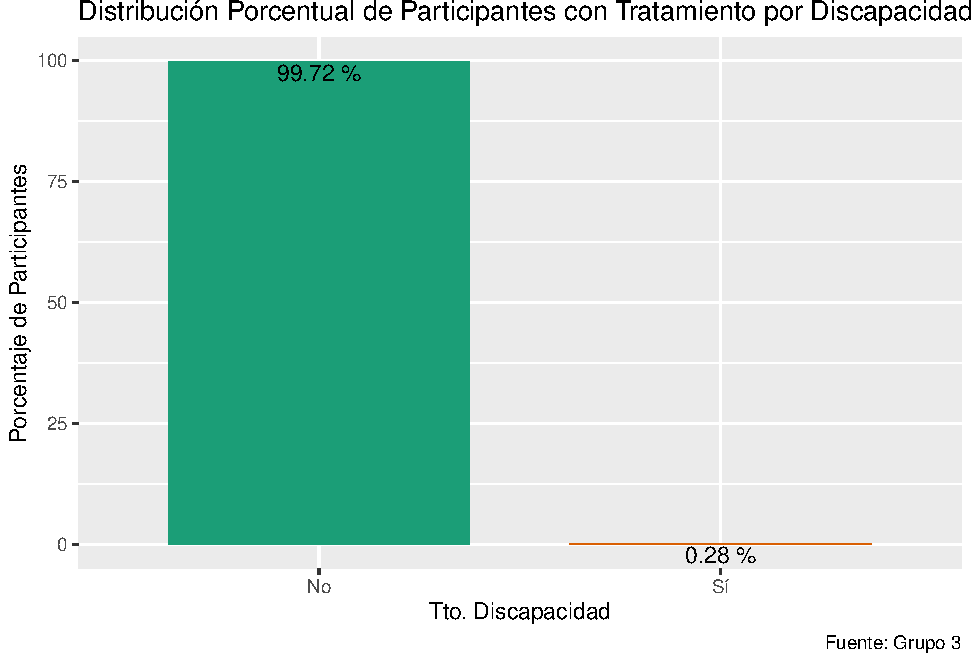
\includegraphics{Info_Dinix_02_files/figure-latex/30_RTTdisc-1.pdf}

\subsection{Ningún Tratamiento
(RTTnin)}\label{ninguxfan-tratamiento-rttnin}

A continuación, la información acerca de los participantes que no
reciben ningún tratamiento:

\begin{longtable}[]{@{}lrrrr@{}}
\caption{Frecuencias de Ningún Tto.}\tabularnewline
\toprule\noalign{}
Ningún Tto. & N & \% & N Acum. & \% Acum. \\
\midrule\noalign{}
\endfirsthead
\toprule\noalign{}
Ningún Tto. & N & \% & N Acum. & \% Acum. \\
\midrule\noalign{}
\endhead
\bottomrule\noalign{}
\endlastfoot
Sí & 1012 & 93.27 & 1012 & 93.27 \\
No & 73 & 6.73 & 1085 & 100.00 \\
\end{longtable}

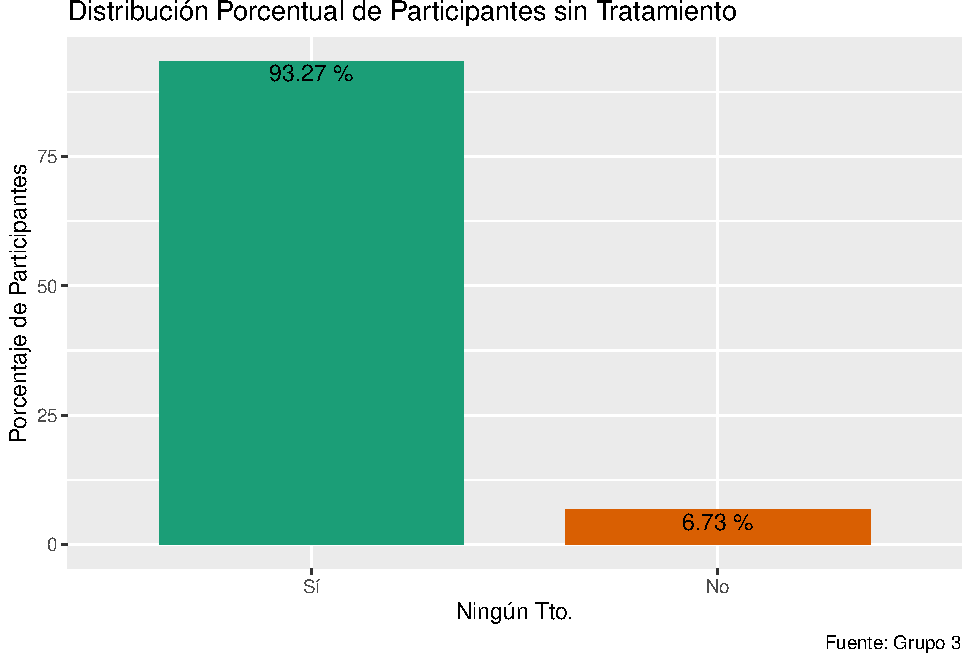
\includegraphics{Info_Dinix_02_files/figure-latex/30_RTTnin-1.pdf}

\subsection{Instrucción Previa al Nivel 3
(Insant3a)}\label{instrucciuxf3n-previa-al-nivel-3-insant3a}

A continuación, la información acerca de los participantes que no
reciben ningún tratamiento:

\begin{longtable}[]{@{}lrrrr@{}}
\caption{Frecuencias de Instruc. Previa}\tabularnewline
\toprule\noalign{}
Instruc. Previa & N & \% & N Acum. & \% Acum. \\
\midrule\noalign{}
\endfirsthead
\toprule\noalign{}
Instruc. Previa & N & \% & N Acum. & \% Acum. \\
\midrule\noalign{}
\endhead
\bottomrule\noalign{}
\endlastfoot
No & 723 & 66.64 & 723 & 66.64 \\
Sí & 287 & 26.45 & 1010 & 93.09 \\
NS/NR & 75 & 6.91 & 1085 & 100.00 \\
\end{longtable}

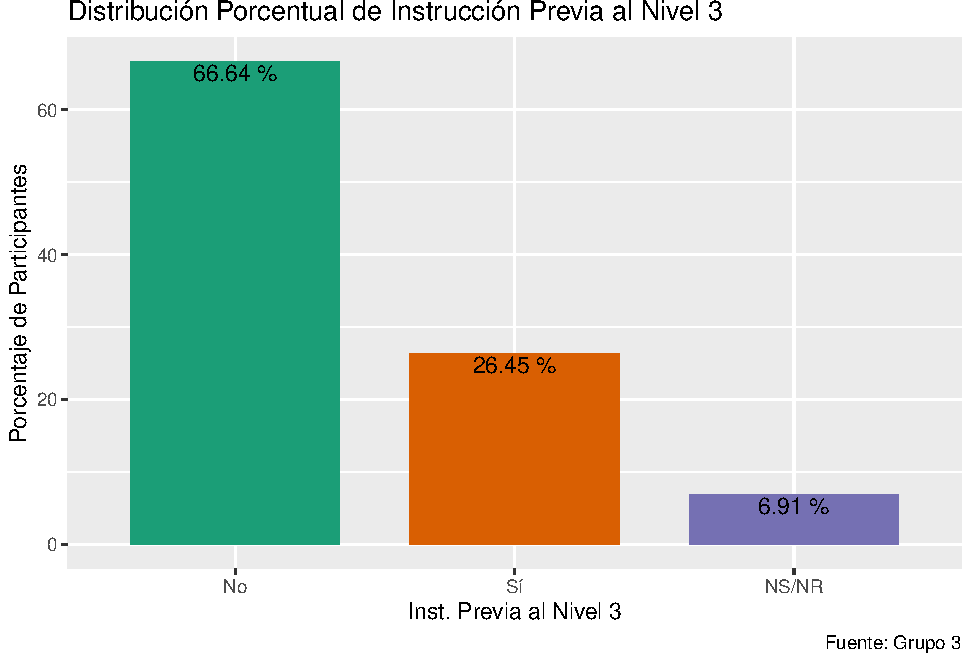
\includegraphics{Info_Dinix_02_files/figure-latex/30_Insant3a-1.pdf}

\section{Análisis Escalar Nivel 3}\label{anuxe1lisis-escalar-nivel-3}

En esta sección pasaremos a analizar la escala DINI en su aplicación al
grupo de Nivel 3.

\subsection{Estructura de Subescalas}\label{estructura-de-subescalas}

\begin{enumerate}
\def\labelenumi{\arabic{enumi}.}
\tightlist
\item
  La subescala ``C'' está compuesta por los ítems C1 a C23 (23 ítems)
\item
  La subescala ``M'' está compuesta por los ítems M1 a M08 (08 ítems)
\item
  La subescala ``S'' está compuesta por los ítems S1 a S13 (13 ítems)
\item
  La subescala ``D'' está compuesta por los ítems D1 a D06 (06 ítems)
\end{enumerate}

Iniciaremos con el análisis de normalidad de las subescalas.

\subsection{Análisis de Normalidad Escala
DINI}\label{anuxe1lisis-de-normalidad-escala-dini}

\subsubsection{Estadísticos
Descriptivos}\label{estaduxedsticos-descriptivos}

\begin{longtable}[]{@{}lrrrr@{}}
\toprule\noalign{}
Variable & Número.de.Casos & Mediana & Media & Desviación.Estándar \\
\midrule\noalign{}
\endhead
\bottomrule\noalign{}
\endlastfoot
CLEN\_sum & 1021 & 21 & 22.69 & 8.47 \\
CMAT\_sum & 1021 & 15 & 16.71 & 6.78 \\
CDES\_sum & 1021 & 15 & 15.59 & 5.68 \\
CFEX\_sum & 1021 & 18 & 18.48 & 5.84 \\
SHAS\_sum & 1021 & 18 & 18.19 & 5.34 \\
SINT\_sum & 1021 & 9 & 9.38 & 3.63 \\
SEXT\_sum & 1021 & 6 & 7.42 & 3.76 \\
C\_sum & 1021 & 70 & 73.46 & 24.21 \\
M\_sum & 1021 & 27 & 27.32 & 7.51 \\
D\_sum & 1021 & 25 & 25.55 & 5.94 \\
\end{longtable}

\subsubsection{Histogramas}\label{histogramas}

Veamos el histograma de cada variable:

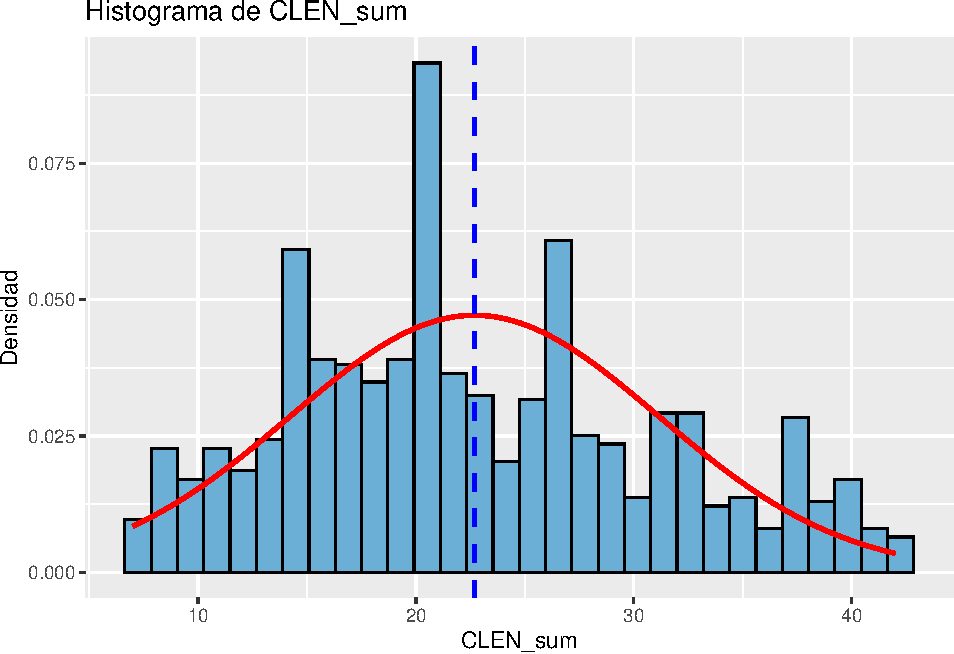
\includegraphics{Info_Dinix_02_files/figure-latex/30_Histos-1.pdf}
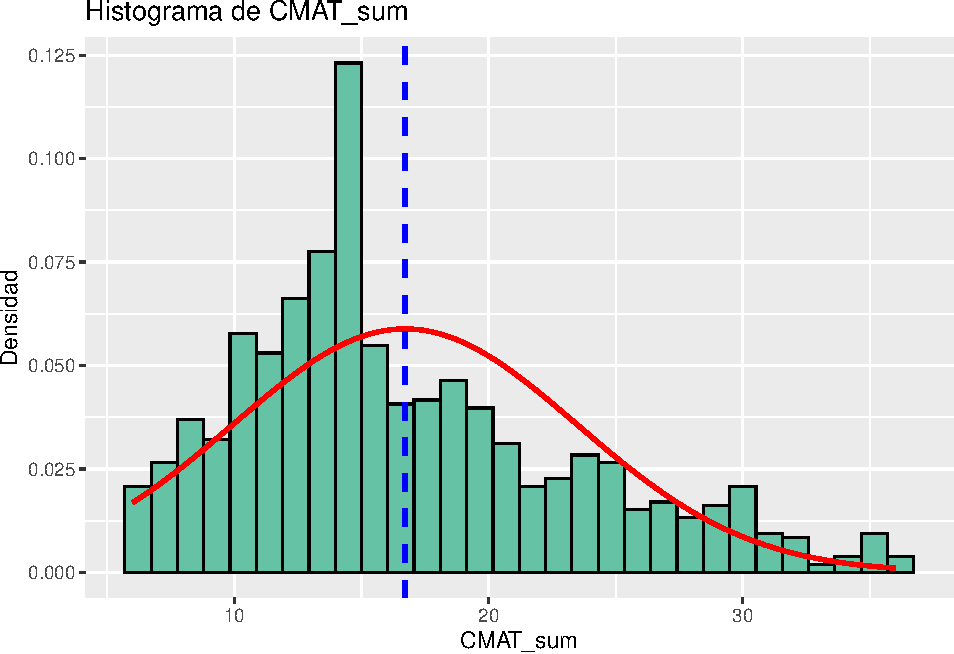
\includegraphics{Info_Dinix_02_files/figure-latex/30_Histos-2.pdf}
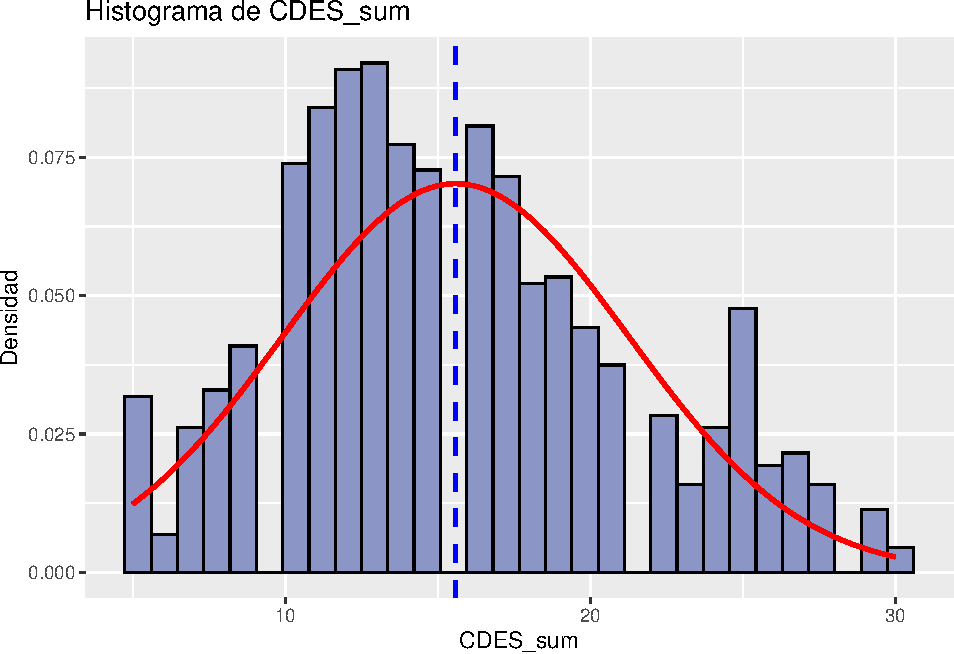
\includegraphics{Info_Dinix_02_files/figure-latex/30_Histos-3.pdf}
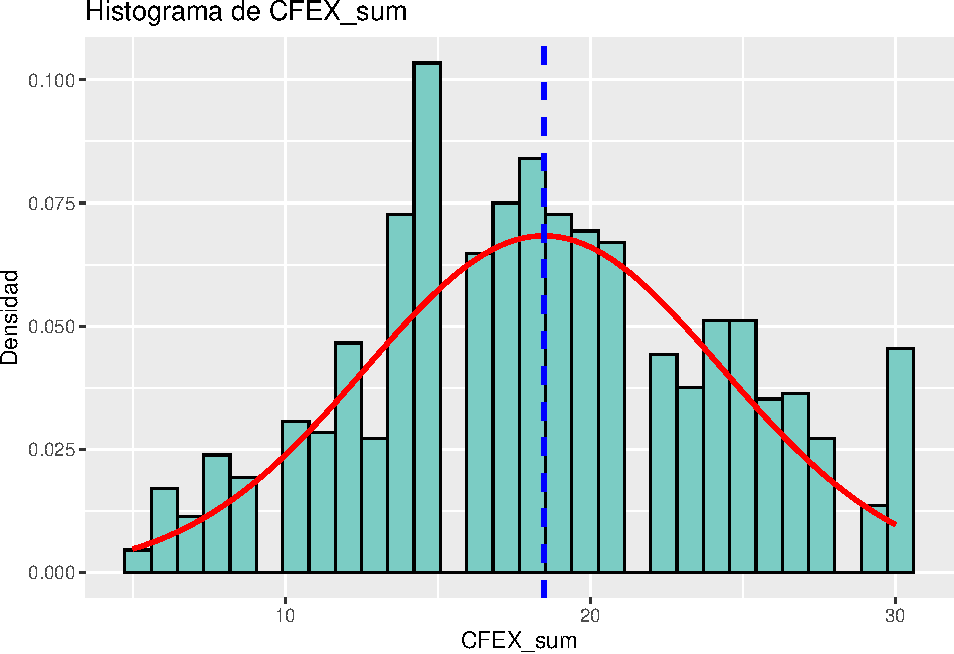
\includegraphics{Info_Dinix_02_files/figure-latex/30_Histos-4.pdf}
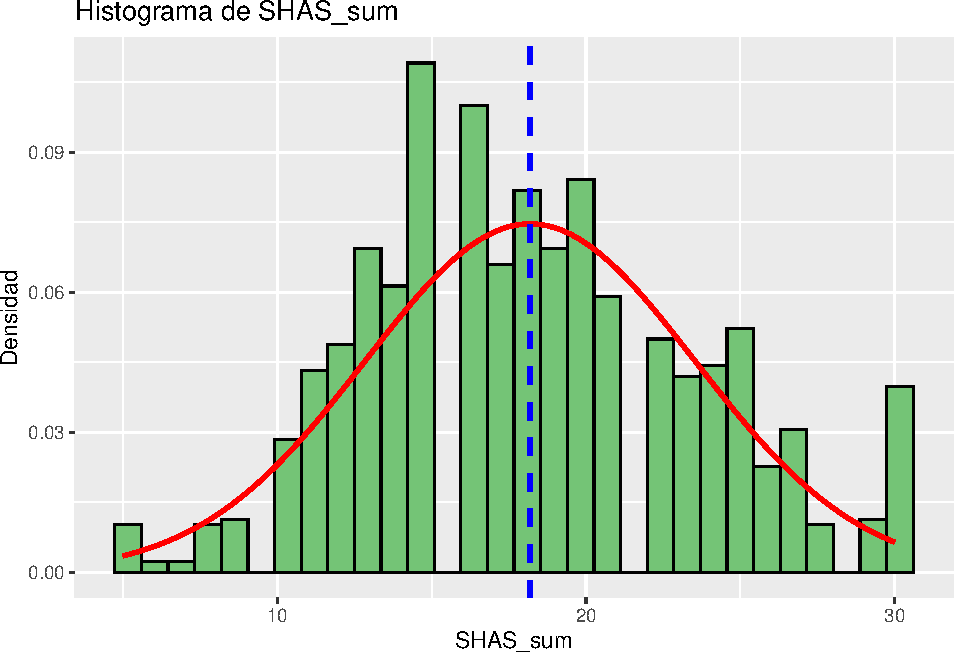
\includegraphics{Info_Dinix_02_files/figure-latex/30_Histos-5.pdf}
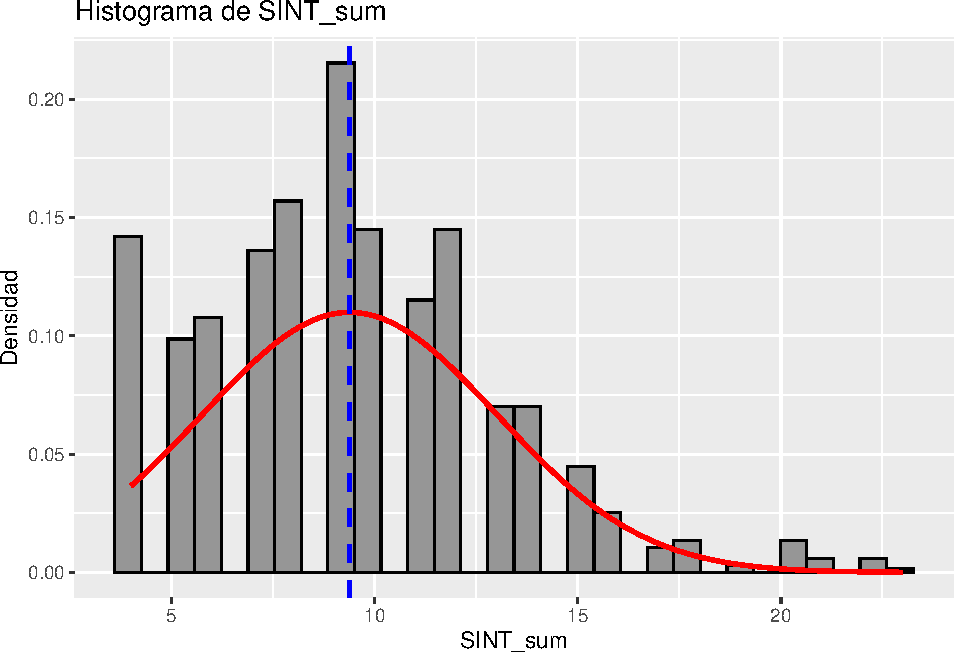
\includegraphics{Info_Dinix_02_files/figure-latex/30_Histos-6.pdf}
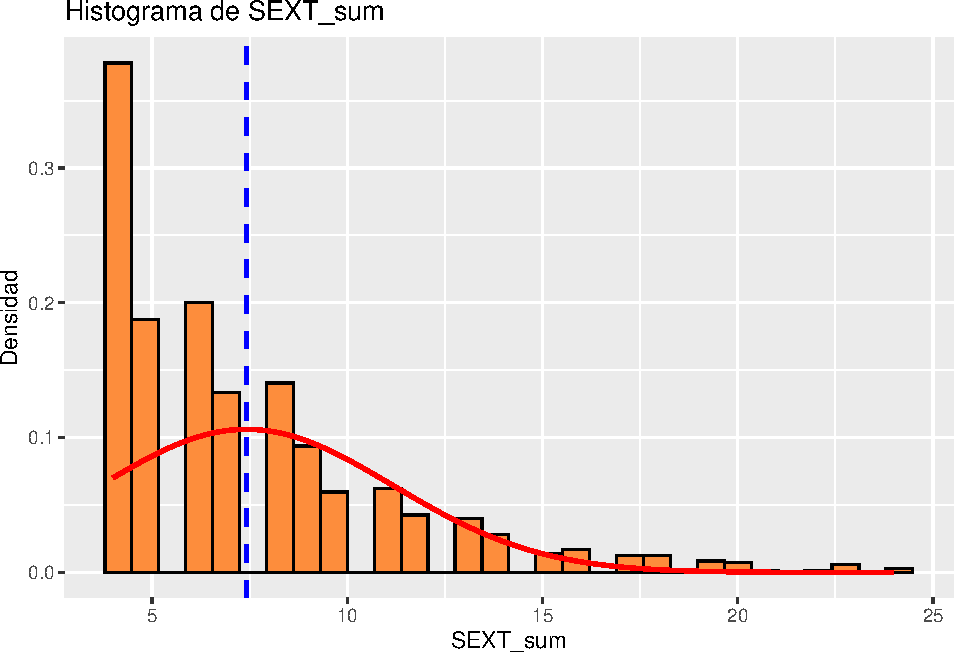
\includegraphics{Info_Dinix_02_files/figure-latex/30_Histos-7.pdf}
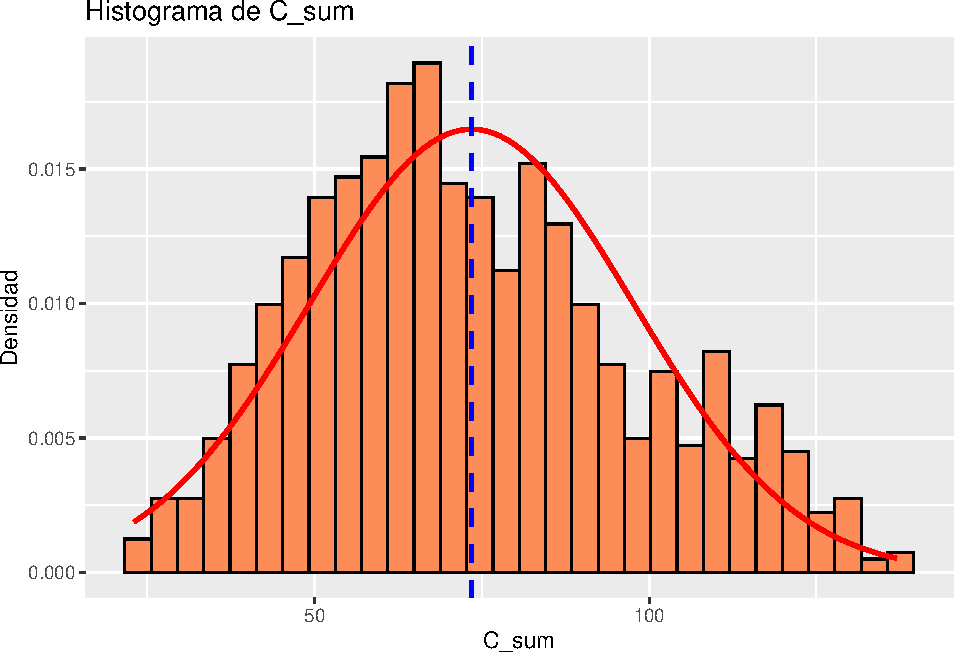
\includegraphics{Info_Dinix_02_files/figure-latex/30_Histos-8.pdf}
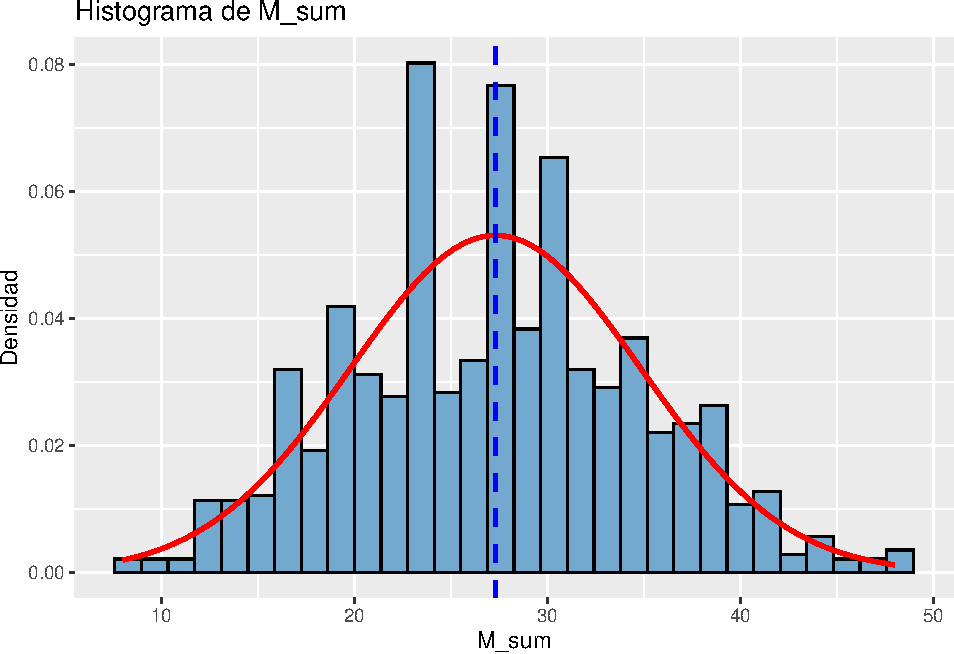
\includegraphics{Info_Dinix_02_files/figure-latex/30_Histos-9.pdf}
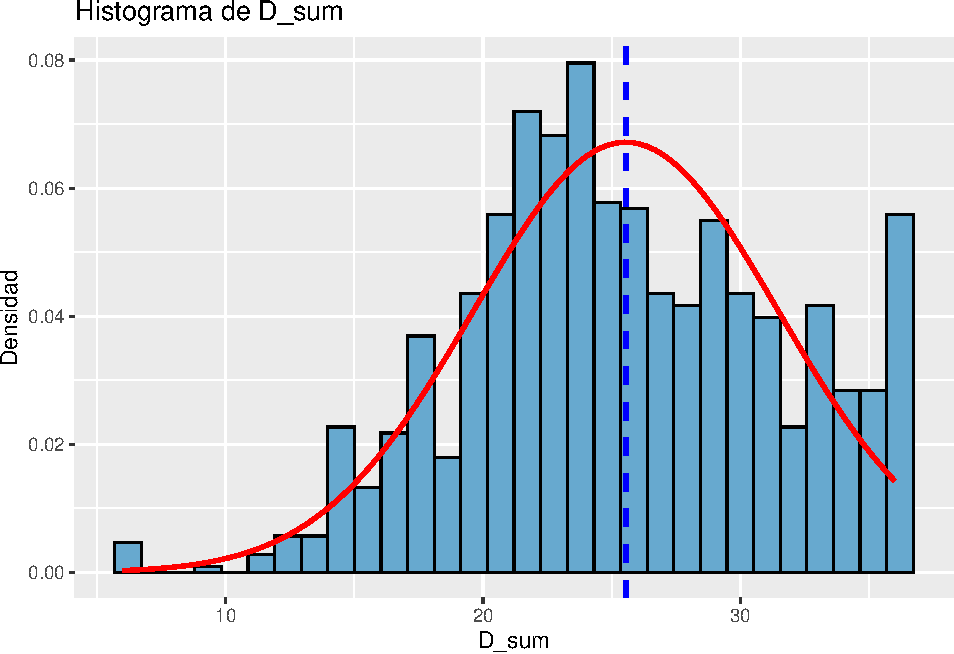
\includegraphics{Info_Dinix_02_files/figure-latex/30_Histos-10.pdf}

\subsubsection{Normalidad}\label{normalidad}

Empezaremos por hacer una comparación gráfica de la distribución de las
subescalas y la distribución normal hipotética.

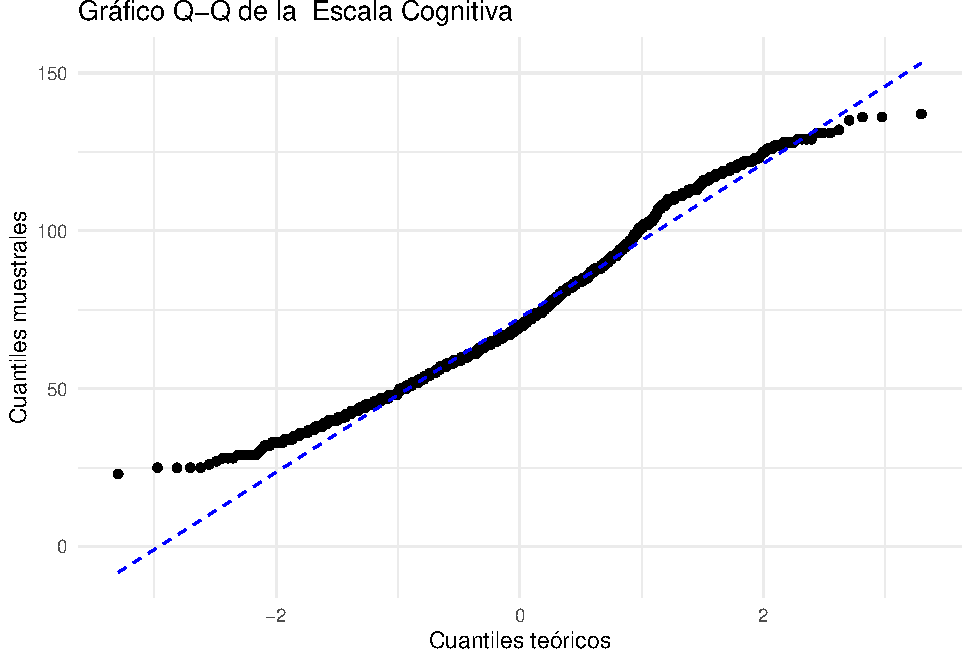
\includegraphics{Info_Dinix_02_files/figure-latex/30_QQ-1.pdf}
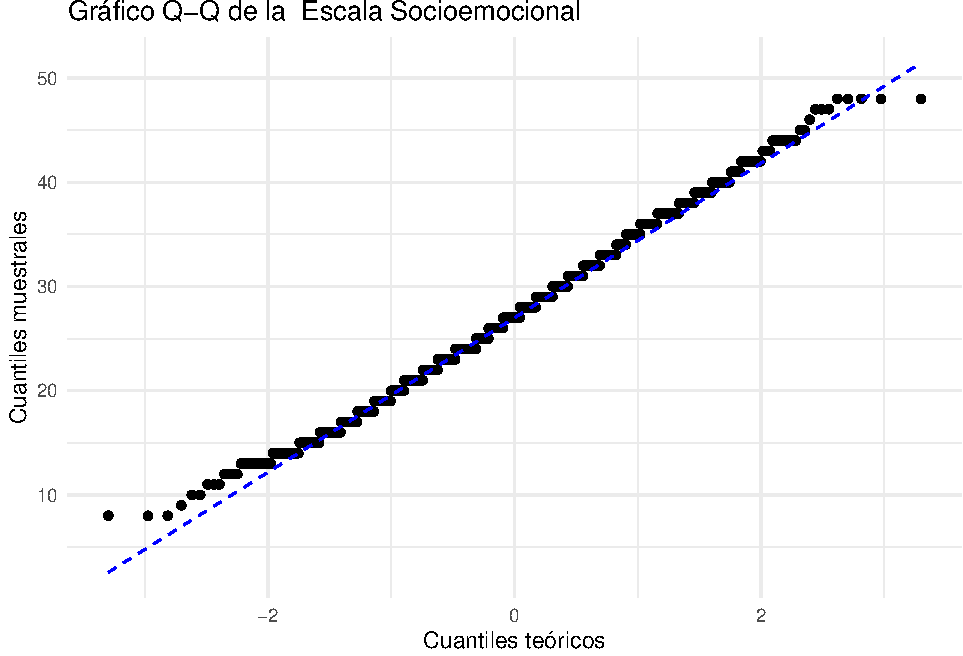
\includegraphics{Info_Dinix_02_files/figure-latex/30_QQ-2.pdf}
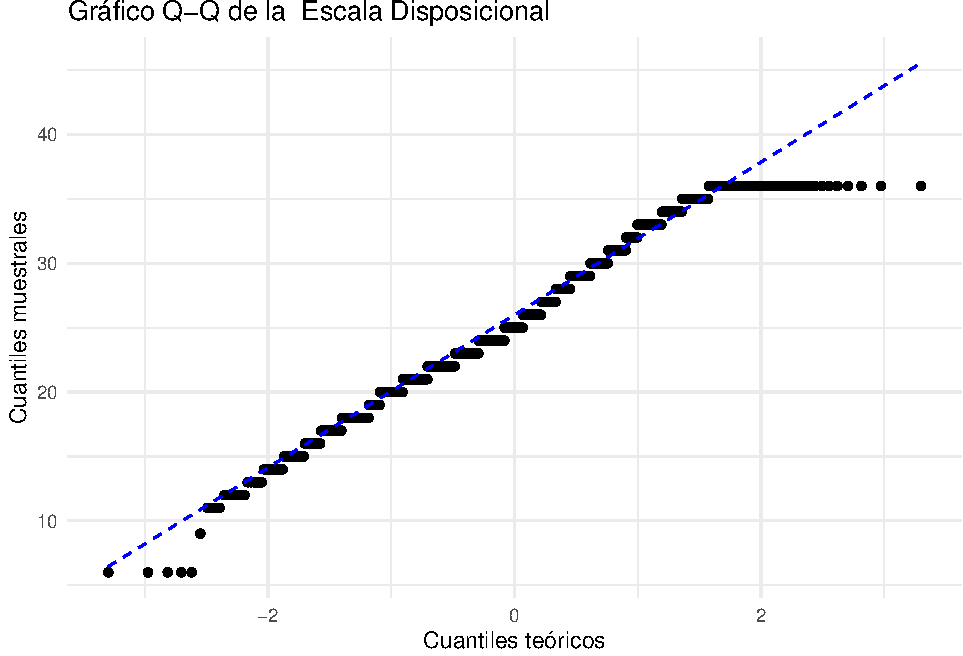
\includegraphics{Info_Dinix_02_files/figure-latex/30_QQ-3.pdf}

Pasemos a calcular los estadísticos de normalidad correspondientes a las
subescalas DINI:

\begin{longtable}[]{@{}
  >{\raggedright\arraybackslash}p{(\columnwidth - 4\tabcolsep) * \real{0.0909}}
  >{\raggedleft\arraybackslash}p{(\columnwidth - 4\tabcolsep) * \real{0.4545}}
  >{\raggedright\arraybackslash}p{(\columnwidth - 4\tabcolsep) * \real{0.4545}}@{}}
\caption{Resultados de los tests de normalidad (S-W, Lilliefors
K-S)}\tabularnewline
\toprule\noalign{}
\begin{minipage}[b]{\linewidth}\raggedright
\end{minipage} & \begin{minipage}[b]{\linewidth}\raggedleft
Shapiro\_Wilk
\end{minipage} & \begin{minipage}[b]{\linewidth}\raggedright
Lilliefors\_KS
\end{minipage} \\
\midrule\noalign{}
\endfirsthead
\toprule\noalign{}
\begin{minipage}[b]{\linewidth}\raggedright
\end{minipage} & \begin{minipage}[b]{\linewidth}\raggedleft
Shapiro\_Wilk
\end{minipage} & \begin{minipage}[b]{\linewidth}\raggedright
Lilliefors\_KS
\end{minipage} \\
\midrule\noalign{}
\endhead
\bottomrule\noalign{}
\endlastfoot
CLEN\_sum & p = 0.00 *** (No se puede asumir normalidad) & p = 0.00 ***
(No se puede asumir normalidad) \\
CMAT\_sum & p = 0.00 *** (No se puede asumir normalidad) & p = 0.00 ***
(No se puede asumir normalidad) \\
CDES\_sum & p = 0.00 *** (No se puede asumir normalidad) & p = 0.00 ***
(No se puede asumir normalidad) \\
CFEX\_sum & p = 0.00 *** (No se puede asumir normalidad) & p = 0.00 ***
(No se puede asumir normalidad) \\
SHAS\_sum & p = 0.00 *** (No se puede asumir normalidad) & p = 0.00 ***
(No se puede asumir normalidad) \\
SINT\_sum & p = 0.00 *** (No se puede asumir normalidad) & p = 0.00 ***
(No se puede asumir normalidad) \\
SEXT\_sum & p = 0.00 *** (No se puede asumir normalidad) & p = 0.00 ***
(No se puede asumir normalidad) \\
C\_sum & p = 0.00 *** (No se puede asumir normalidad) & p = 0.00 *** (No
se puede asumir normalidad) \\
M\_sum & p = 0.00 ** (No se puede asumir normalidad) & p = 0.00 *** (No
se puede asumir normalidad) \\
D\_sum & p = 0.00 *** (No se puede asumir normalidad) & p = 0.00 *** (No
se puede asumir normalidad) \\
\end{longtable}

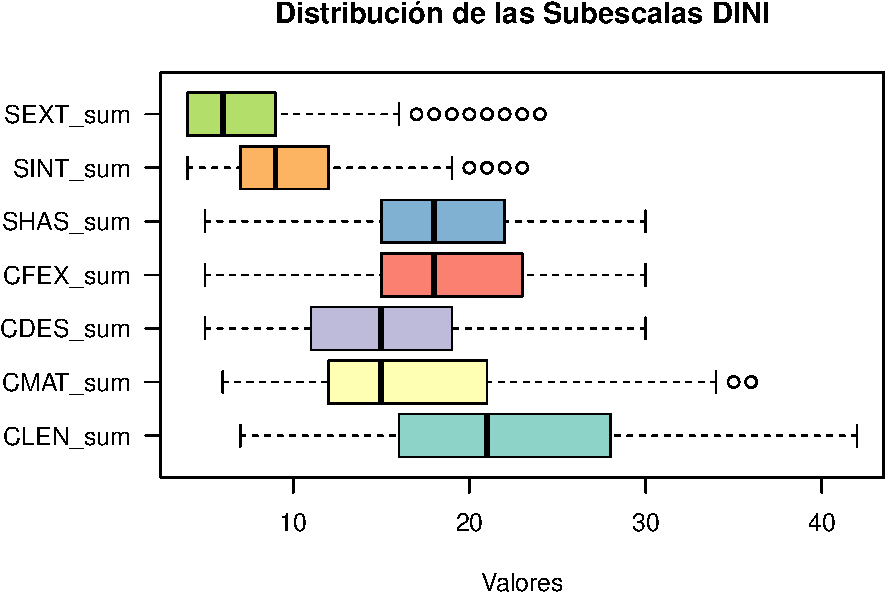
\includegraphics{Info_Dinix_02_files/figure-latex/30_Norma-1.pdf}

\subsubsection{Confiabilidad}\label{confiabilidad}

Pasemos ahora a calcular los índices de confiabilidad alpha de Cronbach
para las subescalas DINI.

\begin{longtable}[]{@{}
  >{\raggedleft\arraybackslash}p{(\columnwidth - 4\tabcolsep) * \real{0.0943}}
  >{\raggedleft\arraybackslash}p{(\columnwidth - 4\tabcolsep) * \real{0.2736}}
  >{\raggedright\arraybackslash}p{(\columnwidth - 4\tabcolsep) * \real{0.6321}}@{}}
\caption{Confiabilidad de la Escala C}\tabularnewline
\toprule\noalign{}
\begin{minipage}[b]{\linewidth}\raggedleft
Std.Alpha
\end{minipage} & \begin{minipage}[b]{\linewidth}\raggedleft
Cantidad.Items.Prescindibles
\end{minipage} & \begin{minipage}[b]{\linewidth}\raggedright
Items
\end{minipage} \\
\midrule\noalign{}
\endfirsthead
\toprule\noalign{}
\begin{minipage}[b]{\linewidth}\raggedleft
Std.Alpha
\end{minipage} & \begin{minipage}[b]{\linewidth}\raggedleft
Cantidad.Items.Prescindibles
\end{minipage} & \begin{minipage}[b]{\linewidth}\raggedright
Items
\end{minipage} \\
\midrule\noalign{}
\endhead
\bottomrule\noalign{}
\endlastfoot
0.96 & 0 & no hay ítems cuya exclusión incremente alpha en más de 0.05
puntos \\
\end{longtable}

\begin{longtable}[]{@{}
  >{\raggedleft\arraybackslash}p{(\columnwidth - 4\tabcolsep) * \real{0.0943}}
  >{\raggedleft\arraybackslash}p{(\columnwidth - 4\tabcolsep) * \real{0.2736}}
  >{\raggedright\arraybackslash}p{(\columnwidth - 4\tabcolsep) * \real{0.6321}}@{}}
\caption{Confiabilidad de la Escala M}\tabularnewline
\toprule\noalign{}
\begin{minipage}[b]{\linewidth}\raggedleft
Std.Alpha
\end{minipage} & \begin{minipage}[b]{\linewidth}\raggedleft
Cantidad.Items.Prescindibles
\end{minipage} & \begin{minipage}[b]{\linewidth}\raggedright
Items
\end{minipage} \\
\midrule\noalign{}
\endfirsthead
\toprule\noalign{}
\begin{minipage}[b]{\linewidth}\raggedleft
Std.Alpha
\end{minipage} & \begin{minipage}[b]{\linewidth}\raggedleft
Cantidad.Items.Prescindibles
\end{minipage} & \begin{minipage}[b]{\linewidth}\raggedright
Items
\end{minipage} \\
\midrule\noalign{}
\endhead
\bottomrule\noalign{}
\endlastfoot
0.84 & 0 & no hay ítems cuya exclusión incremente alpha en más de 0.05
puntos \\
\end{longtable}

\begin{longtable}[]{@{}
  >{\raggedleft\arraybackslash}p{(\columnwidth - 4\tabcolsep) * \real{0.0943}}
  >{\raggedleft\arraybackslash}p{(\columnwidth - 4\tabcolsep) * \real{0.2736}}
  >{\raggedright\arraybackslash}p{(\columnwidth - 4\tabcolsep) * \real{0.6321}}@{}}
\caption{Confiabilidad de la Escala S}\tabularnewline
\toprule\noalign{}
\begin{minipage}[b]{\linewidth}\raggedleft
Std.Alpha
\end{minipage} & \begin{minipage}[b]{\linewidth}\raggedleft
Cantidad.Items.Prescindibles
\end{minipage} & \begin{minipage}[b]{\linewidth}\raggedright
Items
\end{minipage} \\
\midrule\noalign{}
\endfirsthead
\toprule\noalign{}
\begin{minipage}[b]{\linewidth}\raggedleft
Std.Alpha
\end{minipage} & \begin{minipage}[b]{\linewidth}\raggedleft
Cantidad.Items.Prescindibles
\end{minipage} & \begin{minipage}[b]{\linewidth}\raggedright
Items
\end{minipage} \\
\midrule\noalign{}
\endhead
\bottomrule\noalign{}
\endlastfoot
0.8 & 0 & No hay ítems cuya exclusión incremente alpha en más de 0.05
puntos \\
\end{longtable}

\begin{longtable}[]{@{}
  >{\raggedleft\arraybackslash}p{(\columnwidth - 4\tabcolsep) * \real{0.0943}}
  >{\raggedleft\arraybackslash}p{(\columnwidth - 4\tabcolsep) * \real{0.2736}}
  >{\raggedright\arraybackslash}p{(\columnwidth - 4\tabcolsep) * \real{0.6321}}@{}}
\caption{Confiabilidad de la Escala D}\tabularnewline
\toprule\noalign{}
\begin{minipage}[b]{\linewidth}\raggedleft
Std.Alpha
\end{minipage} & \begin{minipage}[b]{\linewidth}\raggedleft
Cantidad.Items.Prescindibles
\end{minipage} & \begin{minipage}[b]{\linewidth}\raggedright
Items
\end{minipage} \\
\midrule\noalign{}
\endfirsthead
\toprule\noalign{}
\begin{minipage}[b]{\linewidth}\raggedleft
Std.Alpha
\end{minipage} & \begin{minipage}[b]{\linewidth}\raggedleft
Cantidad.Items.Prescindibles
\end{minipage} & \begin{minipage}[b]{\linewidth}\raggedright
Items
\end{minipage} \\
\midrule\noalign{}
\endhead
\bottomrule\noalign{}
\endlastfoot
0.87 & 0 & no hay ítems cuya exclusión incremente alpha en más de 0.05
puntos \\
\end{longtable}

De los índices obtenidos podemos establecer que las subescalas DINI
muestran una gran confiabilidad; es decir, miden de forma consistente,
sin que exista ítems que vayan en detrimento de la confiabilidad
general. Por el contrario, todos los reactivos ostentan consistencia con
los demás.

\subsubsection{Análisis Factorial}\label{anuxe1lisis-factorial}

Pasaremos a evaluar la validez de la Escala DINI en su aplicación a la
muestra peruana 2024.

En el contexto de uso del análisis psicométrico de esta escala, el
objetivo es corroborar que la estructura de las variables a evaluar se
ha mantenido constante en esta aplicación.

Debido a que estamos analizando una escala ya construida y validada en
su población original (Uruguay), nuestra tarea en este punto es
establecer si la estructura factorial del instrumento se reproduce
razonablemente bien en nuestra muestra proveniente de la población
peruana.

A fin de determinar esto, procederemos a realizar la variante llamada
Análisis Factorial Confirmatorio (AFC).

lavaan 0.6-19 ended normally after 59 iterations

Estimator ML Optimization method NLMINB Number of model parameters 106

Number of observations 1021

Model Test User Model:

Test statistic 10317.985 Degrees of freedom 1169 P-value (Chi-square)
0.000

Model Test Baseline Model:

Test statistic 36939.287 Degrees of freedom 1225 P-value 0.000

User Model versus Baseline Model:

Comparative Fit Index (CFI) 0.744 Tucker-Lewis Index (TLI) 0.732

Loglikelihood and Information Criteria:

Loglikelihood user model (H0) -73943.650 Loglikelihood unrestricted
model (H1) NA

Akaike (AIC) 148099.299 Bayesian (BIC) 148621.724 Sample-size adjusted
Bayesian (SABIC) 148285.058

Root Mean Square Error of Approximation:

RMSEA 0.088 90 Percent confidence interval - lower 0.086 90 Percent
confidence interval - upper 0.089 P-value H\_0: RMSEA \textless= 0.050
0.000 P-value H\_0: RMSEA \textgreater= 0.080 1.000

Standardized Root Mean Square Residual:

SRMR 0.081

Parameter Estimates:

Standard errors Standard Information Expected Information saturated (h1)
model Structured

Latent Variables: Estimate Std.Err z-value
P(\textgreater\textbar z\textbar) Std.lv Std.all Cognitivo
=\textasciitilde{}\\
C1 1.000 1.234 0.835 C2 0.935 0.029 32.139 0.000 1.154 0.811 C3 0.757
0.032 23.431 0.000 0.933 0.650 C4 0.898 0.029 30.950 0.000 1.108 0.791
C5 1.042 0.032 32.442 0.000 1.285 0.816 C6 0.929 0.029 32.366 0.000
1.146 0.814 C7 0.865 0.028 31.385 0.000 1.067 0.799 C8 0.784 0.030
26.186 0.000 0.967 0.706 C9 0.822 0.028 28.967 0.000 1.014 0.757 C10
1.004 0.029 34.929 0.000 1.238 0.853 C11 0.838 0.030 28.348 0.000 1.034
0.746 C12 0.629 0.030 20.751 0.000 0.776 0.591 C13 0.466 0.026 18.120
0.000 0.575 0.528 C14 0.760 0.031 24.749 0.000 0.937 0.677 C15 0.825
0.029 28.477 0.000 1.017 0.749 C16 0.727 0.031 23.441 0.000 0.897 0.650
C17 0.892 0.034 26.599 0.000 1.100 0.714 C18 0.931 0.035 26.539 0.000
1.149 0.713 C19 0.724 0.032 22.871 0.000 0.893 0.638 C20 0.937 0.030
30.868 0.000 1.156 0.790 C21 0.846 0.026 32.475 0.000 1.044 0.816 C22
0.861 0.028 31.291 0.000 1.062 0.797 C23 0.799 0.029 27.881 0.000 0.985
0.738 Motor =\textasciitilde{}\\
M1 1.000 0.712 0.489 M2 1.421 0.095 14.901 0.000 1.012 0.720 M3 0.976
0.081 11.998 0.000 0.695 0.488 M4 1.138 0.080 14.216 0.000 0.811 0.653
M5 1.400 0.093 15.108 0.000 0.997 0.742 M6 1.111 0.083 13.404 0.000
0.791 0.586 M7 1.170 0.081 14.402 0.000 0.833 0.670 M8 1.381 0.094
14.711 0.000 0.983 0.700 Socioemocional =\textasciitilde{}\\
S1 1.000 1.015 0.782 S2 1.085 0.041 26.515 0.000 1.101 0.792 S3 -0.313
0.042 -7.535 0.000 -0.318 -0.247 S4 -0.448 0.037 -12.254 0.000 -0.455
-0.395 S5 -0.470 0.039 -12.109 0.000 -0.477 -0.390 S6 -0.384 0.035
-10.977 0.000 -0.389 -0.355 S7 0.844 0.042 20.302 0.000 0.857 0.629 S8
1.035 0.040 25.711 0.000 1.050 0.772 S9 0.820 0.043 19.166 0.000 0.832
0.598 S10 -0.163 0.047 -3.466 0.001 -0.166 -0.114 S11 -0.223 0.036
-6.149 0.000 -0.226 -0.202 S12 -0.396 0.033 -11.888 0.000 -0.402 -0.384
S13 -0.455 0.043 -10.453 0.000 -0.462 -0.339 Disposicional
=\textasciitilde{}\\
D1 1.000 0.929 0.758 D2 0.784 0.042 18.533 0.000 0.728 0.582 D3 1.102
0.040 27.258 0.000 1.023 0.823 D4 0.985 0.042 23.244 0.000 0.915 0.715
D5 0.925 0.041 22.600 0.000 0.860 0.697 D6 1.164 0.044 26.217 0.000
1.082 0.795

Covariances: Estimate Std.Err z-value P(\textgreater\textbar z\textbar)
Std.lv Std.all Cognitivo \textasciitilde\textasciitilde{}\\
Motor 0.774 0.061 12.702 0.000 0.881 0.881 Socioemocional 0.862 0.057
15.084 0.000 0.688 0.688 Disposicional 0.932 0.057 16.254 0.000 0.813
0.813 Motor \textasciitilde\textasciitilde{}\\
Socioemocional 0.521 0.045 11.661 0.000 0.721 0.721 Disposicional 0.521
0.044 11.930 0.000 0.787 0.787 Socioemocional
\textasciitilde\textasciitilde{}\\
Disposicional 0.795 0.050 15.820 0.000 0.843 0.843

Variances: Estimate Std.Err z-value P(\textgreater\textbar z\textbar)
Std.lv Std.all .C1 0.663 0.031 21.095 0.000 0.663 0.303 .C2 0.694 0.033
21.342 0.000 0.694 0.343 .C3 1.192 0.054 22.117 0.000 1.192 0.578 .C4
0.733 0.034 21.500 0.000 0.733 0.374 .C5 0.832 0.039 21.297 0.000 0.832
0.335 .C6 0.667 0.031 21.308 0.000 0.667 0.337 .C7 0.647 0.030 21.445
0.000 0.647 0.362 .C8 0.943 0.043 21.947 0.000 0.943 0.502 .C9 0.764
0.035 21.716 0.000 0.764 0.426 .C10 0.574 0.028 20.847 0.000 0.574 0.272
.C11 0.850 0.039 21.774 0.000 0.850 0.443 .C12 1.125 0.051 22.245 0.000
1.125 0.651 .C13 0.854 0.038 22.342 0.000 0.854 0.721 .C14 1.038 0.047
22.042 0.000 1.038 0.541 .C15 0.812 0.037 21.762 0.000 0.812 0.440 .C16
1.098 0.050 22.117 0.000 1.098 0.577 .C17 1.166 0.053 21.917 0.000 1.166
0.491 .C18 1.280 0.058 21.921 0.000 1.280 0.492 .C19 1.163 0.053 22.147
0.000 1.163 0.593 .C20 0.804 0.037 21.510 0.000 0.804 0.376 .C21 0.547
0.026 21.292 0.000 0.547 0.334 .C22 0.648 0.030 21.457 0.000 0.648 0.365
.C23 0.813 0.037 21.815 0.000 0.813 0.456 .M1 1.615 0.074 21.845 0.000
1.615 0.761 .M2 0.954 0.048 19.986 0.000 0.954 0.482 .M3 1.544 0.071
21.847 0.000 1.544 0.762 .M4 0.883 0.042 20.801 0.000 0.883 0.573 .M5
0.812 0.041 19.610 0.000 0.812 0.450 .M6 1.199 0.056 21.343 0.000 1.199
0.657 .M7 0.851 0.041 20.626 0.000 0.851 0.551 .M8 1.006 0.050 20.266
0.000 1.006 0.510 .S1 0.655 0.035 18.483 0.000 0.655 0.389 .S2 0.721
0.040 18.192 0.000 0.721 0.373 .S3 1.564 0.070 22.428 0.000 1.564 0.939
.S4 1.121 0.051 22.119 0.000 1.121 0.844 .S5 1.263 0.057 22.131 0.000
1.263 0.848 .S6 1.048 0.047 22.222 0.000 1.048 0.874 .S7 1.119 0.054
20.898 0.000 1.119 0.604 .S8 0.750 0.040 18.752 0.000 0.750 0.405 .S9
1.245 0.059 21.157 0.000 1.245 0.643 .S10 2.073 0.092 22.560 0.000 2.073
0.987 .S11 1.208 0.054 22.485 0.000 1.208 0.959 .S12 0.938 0.042 22.150
0.000 0.938 0.853 .S13 1.639 0.074 22.260 0.000 1.639 0.885 .D1 0.640
0.032 19.806 0.000 0.640 0.426 .D2 1.034 0.048 21.547 0.000 1.034 0.661
.D3 0.499 0.027 18.215 0.000 0.499 0.323 .D4 0.799 0.039 20.440 0.000
0.799 0.489 .D5 0.780 0.038 20.648 0.000 0.780 0.514 .D6 0.680 0.036
19.019 0.000 0.680 0.367 Cognitivo 1.522 0.093 16.395 0.000 1.000 1.000
Motor 0.507 0.064 7.951 0.000 1.000 1.000 Socioemocional 1.031 0.072
14.371 0.000 1.000 1.000 Disposicional 0.863 0.062 13.885 0.000 1.000
1.000

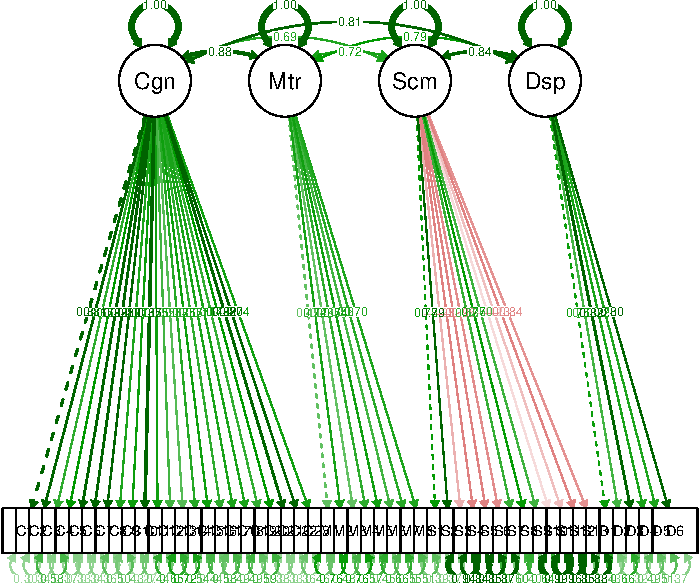
\includegraphics{Info_Dinix_02_files/figure-latex/30_AFC-1.pdf}

\end{document}
